\documentclass[12pt,oneside]{uhthesis}
\usepackage{subfigure}
\usepackage[ruled,lined,linesnumbered,titlenumbered,algochapter,spanish,onelanguage]{algorithm2e}
\usepackage{amsmath}
\usepackage{amssymb}
\usepackage{amsbsy}
\usepackage{caption,booktabs}
\captionsetup{ justification = centering }
%\usepackage{mathpazo}
\usepackage[spanish]{babel}
\usepackage{float}
\setlength{\marginparwidth}{2cm}
\usepackage{todonotes}
\usepackage{listings}
\usepackage{xcolor}
\usepackage{multicol}
\usepackage{graphicx}
\floatstyle{plaintop}
\restylefloat{table}

\usepackage{tabularx}
\usepackage[table]{xcolor}
\usepackage{booktabs}
\usepackage{array}
\usepackage{tikz}
\usepackage{subcaption} 
\usepackage[utf8]{inputenc} % Codificación UTF-8
\usepackage[T1]{fontenc}    % Codificación de fuentes
\usetikzlibrary{shapes.geometric, arrows, positioning}

% --- Estilosde tikz ---
\tikzstyle{startstop} = [rectangle, rounded corners, minimum width=3cm, minimum height=0.5cm,text centered, draw=black, fill=gray!20]
\tikzstyle{io} = [trapezium, trapezium left angle=70, trapezium right angle=110, minimum width=1.5cm, minimum height=0.5cm, text centered, draw=black, fill=blue!10]
\tikzstyle{process} = [rectangle, minimum width=3cm, minimum height=1cm, text centered, draw=black, fill=orange!10]
\tikzstyle{decision} = [rectangle, minimum width=1cm, minimum height=1cm, text centered, draw=black, fill=green!10]

\tikzstyle{arrow} = [thick,->,>=stealth']
% --- Estilos de tikz ---


\addbibresource{Bibliography.bib}
% \setlength{\parskip}{\baselineskip}%
\renewcommand{\tablename}{Tabla}
\renewcommand{\listalgorithmcfname}{Índice de Algoritmos}
%\dontprintsemicolon
\SetAlgoNoEnd
% Para numerar \subsubsection y que aparezcan en el índice
\setcounter{tocdepth}{4} % Incluir subsubsecciones en el índice
\setcounter{secnumdepth}{4} % Numerar subsubsecciones

\definecolor{codegreen}{rgb}{0,0.6,0}
\definecolor{codegray}{rgb}{0.5,0.5,0.5}
\definecolor{codepurple}{rgb}{0.58,0,0.82}
\definecolor{backcolour}{rgb}{0.95,0.95,0.92}

\lstdefinestyle{mystyle}{
    backgroundcolor=\color{backcolour},   
    commentstyle=\color{codegreen},
    keywordstyle=\color{purple},
    numberstyle=\tiny\color{codegray},
    stringstyle=\color{codepurple},
    basicstyle=\ttfamily\footnotesize,
    breakatwhitespace=false,         
    breaklines=true,                 
    captionpos=b,                    
    keepspaces=true,                 
    numbers=left,                    
    numbersep=5pt,                  
    showspaces=false,                
    showstringspaces=false,
    showtabs=false,                  
    tabsize=4
}

\lstset{style=mystyle}

\title{Implementación de una API de autenticación gráfica basada en Passpoints}

\degree{Licenciado en  Ciencias de la Computación}

\author{\\\vspace{0.25cm}Alex Sánchez Saez}
\advisor{\\\vspace{0.25cm}MSc. Joaquín Alberto Herrera Macías\\\vspace{0.25cm}MSc. Evaristo José Madarro Capó\\\vspace{0.25cm}MSc. Lisset Suárez Plasencia}

\faculty{Facultad de Matemática y Computación}
\date{La Habana, \today \vspace{0.25cm}}
\logo{Graphics/uhlogo}
\makenomenclature
\usepackage{adjustbox}
\renewcommand{\vec}[1]{\boldsymbol{#1}}
\newcommand{\diff}[1]{\ensuremath{\mathrm{d}#1}}
\newcommand{\me}[1]{\mathrm{e}^{#1}}
\newcommand{\pf}{\mathfrak{p}}
\newcommand{\qf}{\mathfrak{q}}
%\newcommand{\kf}{\mathfrak{k}}
\newcommand{\kt}{\mathtt{k}}
\newcommand{\mf}{\mathfrak{m}}
\newcommand{\hf}{\mathfrak{h}}
\newcommand{\fac}{\mathrm{fac}}
\newcommand{\maxx}[1]{\max\left\{ #1 \right\} }
\newcommand{\minn}[1]{\min\left\{ #1 \right\} }
\newcommand{\lldpcf}{1.25}
\newcommand{\nnorm}[1]{\left\lvert #1 \right\rvert }
\renewcommand{\lstlistingname}{Ejemplo de código}
\renewcommand{\lstlistlistingname}{Ejemplos de código}

\newcounter{anexofignum}
% Comando personalizado para captions de anexos
\newcommand{\anexofigurecaption}[1]{%
	% Incrementa el contador de anexos
	\refstepcounter{anexofignum}%
	% Anular temporalmente el formato de label definido globalmente
	\captionsetup{labelformat=empty}%
	\caption{Anexo No~\arabic{anexofignum} (figura~\thefigure): #1}%
	% Restaurar el formato por defecto para siguientes captions
	\captionsetup{labelformat=default}%
}


\DeclareCiteCommand{\cite}[\mkbibbrackets]
{\usebibmacro{prenote}}
{\usebibmacro{citeindex}%
	\bibhyperref{\printfield{labelnumber}}} % Agrega hipervínculo a la cita
{\multicitedelim}
{\usebibmacro{postnote}}

\begin{document}

\frontmatter
\maketitle

\begin{dedication}
    Dedicación
\end{dedication}
\begin{acknowledgements}
    Agradecimientos
\end{acknowledgements}
\begin{opinion}
    Opiniones de los tutores
\end{opinion}
\begin{resumen}
	La autenticación es crucial para la protección de los usuarios y sus datos. Debido a las debilidades que aparecen en las contraseñas alfanuméricas por la acción de los usuarios, se han desarrollado nuevos enfoques como son los basados en autenticación gráfica. Uno de estos sistemas es el \textit{Passpoints}, el cual se destaca por su seguridad y facilidad de uso. En este trabajo se presenta una implementación propia de dicho sistema, resultado de un exhaustivo estudio del sistema en cuestión. Dicho estudio abordó tanto el funcionamiento como la seguridad del \textit{Passpoints}, identificando sus debilidades y explorando las propuestas existentes para mitigarlas. Para la implementación principal de este sistema, se llevaron a cabo otras implementaciones intermedias esenciales para su desarrollo completo. Para ello se realizó un análisis exhaustivo de los métodos de discretización disponibles con el fin de seleccionar el más efectivo y eficiente para su posterior traducción a código de programación. Así como una investigación referente a la adaptación de este sistema a la variedad de resoluciones de pantalla y tamaños de imagen actuales, permitiendo la adaptación de esta implementación a cualquier tipo de dispositivo. Este proceso es fundamental para convertir el sistema en un producto real que pueda ser evaluado por usuarios reales en diferentes medios.
\end{resumen}

\begin{abstract}
  Authentication is crucial for protecting users and their data. Due to the weaknesses that appear in alphanumeric passwords as a result of user actions, new approaches have been developed, such as those based on graphical authentication. One of these systems is Passpoints, which stands out for its security and ease of use. This work presents our own implementation of this system, the result of an exhaustive study of the system in question. This study addressed both the functioning and security of thesystem, identifying its weaknesses and exploring existing proposals to mitigate them. For the main implementation of this system, other essential intermediate implementations were carried out for its complete development. To achieve this, a comprehensive analysis of available discretization methods was conducted to select the most effective and efficient for subsequent translation into programming code, as well as research regarding the adaptation of this system to the variety of current screen resolutions and image sizes, allowing the adaptation of this implementation to any type of device. This process is fundamental to turning the system into a real product that can be evaluated by real users across different media.
\end{abstract}


\tableofcontents
\listoffigures
% \listoftables
% \listofalgorithms
\lstlistoflistings

\mainmatter

\chapter*{Introducción}\label{chapter:introduction}
\addcontentsline{toc}{chapter}{Introducción}
Desde la popularización del internet en los años 90, es creciente la tendencia a almacenar enormes cantidades de datos en los distintos servicios en línea, desde comercios electrónicos, redes sociales, aplicaciones bancarias, hasta servicios de \textit{streaming}. Servicios como estos han crecido exponencialmente, así como la cantidad de usuarios que los consumen. 

La necesidad de mantener segura y privada la información de los usuarios, muchas veces sensible, originó el uso de sistemas de autenticación seguros, condicionados al hecho de ser eficientes y fáciles de utilizar. La autenticación es el proceso mediante el cual un sistema verifica la identidad del usuario que intenta acceder a un recurso protegido, por ello constituye un pilar fundamental de la seguridad informática. Existen tres tipos principales de autenticación, basada en tokens, basadas en conocimiento y la autenticación biométrica. Cada uno de estos puede verse como la respuesta a una pregunta, de cara a quien intenta acceder al recurso protegido: ¿qué tienes?, ¿qué sabes? o ¿quién eres?

La autenticación basada en tokens responde a la pregunta: ¿qué tienes?, y se basa en que el usuario posea un token de identidad que demuestre su autenticidad, como, por ejemplo, tarjetas de crédito, llaves físicas y digitales. Uno de los ejemplos más utilizados en diferentes tipos de aplicaciones es JWT (\textit{JSON Web Token})   \cite{massimo_nardone__2023}, que son utilizados sobre todo para conectar un cliente con un servidor web. Este consiste en el uso de un token de acceso que contiene los permisos y datos del usuario al sistema, este token iría codificado en la cabecera de la petición. OAuth  \cite{aravind_ayyagiri__2023} es un protocolo para la autenticación multifactor, usa tokens de vida corta y permisos granulares, lo que reduce el riesgo de robo de credenciales y phishing. Es ampliamente utilizado para la integración de autenticación con redes sociales en distintos tipos de aplicaciones.

¿Quién eres?, es la pregunta cuya respuesta está vinculada a la autenticación biométrica. En esta se pide al usuario que demuestre su identidad a partir de datos que provengan de sí mismo, como pueden ser las huellas dactilares en el conocido Touch ID  \cite{liu_jin__2019}, reconocimientos faciales \cite{nur_dua_fathansyah_atan__2024} y reconocimiento de voz \cite{saquib2011voiceprint}. A pesar de que este tipo de autenticación destaca por su seguridad, tiene la desventaja de requerir hardware especial para su uso. 

Por último, el método más utilizado es el basado en conocimiento, el cual se puede ver como la respuesta a la pregunta ¿qué sabes? Desde hace muchos años, las contraseñas alfanuméricas han sido el estándar en este tipo. Sin embargo, debido a la evolución de la capacidad de cómputo y el desarrollo de diferentes tipos de ataques, como son los ataques de diccionarios  \cite{10.1145/1102120.1102168}, fuerza bruta  \cite{Apostol2012BruteforceA} o rainbow table  \cite{wahab2024investigating}, se ha visto debilitada su seguridad al punto de hacerlas inseguras para el usuario común. Estudios han demostrado que, para los usuarios es difícil recordar contraseñas alfanuméricas con un alto nivel de aleatoriedad y de gran longitud. Creando contraseñas débiles y fáciles de predecir computacionalmente. Esto plantea la necesidad de desarrollar alternativas más robustas y adaptadas a los desafíos actuales. En respuesta a esto se han propuesto las contraseñas gráficas como una alternativa.

La principal diferencia entre las contraseñas gráficas y alfanuméricas reside en la naturaleza de la información a memorizar. En el caso de las alfanuméricas se memorizan conjuntos de caracteres y en el caso de las gráficas se utiliza información visual que es más fácil de recordar por los usuarios. Estudios como  \cite{paivio2013imagery, shepard1967recognition, nelson1976pictorial}  avalan la anterior idea a través de la comparación de la capacidad de memoria visual y verbal, con la demostración de que las imágenes se analizan tanto verbal como visualmente  \cite{shepard1967recognition}, a diferencia de las palabras que se analizan solo verbalmente. Esto sitúa a las contraseñas gráficas como una buena alternativa, más segura y fácil de usar que las alfanuméricas.

Entre los sistemas basados en contraseñas gráficas destaca el \textit{Passpoints}  \cite{wiedenbeck2005passpoints} por su seguridad y usabilidad. Este es un sistema en el que el usuario selecciona 5 puntos ordenados de una imagen. Llevar a cabo la implementación de este sistema, así como analizar su seguridad y resistencia ante ataques es una problemática de interés, pues puede ayudar a mejorar la seguridad de los datos en diferentes aplicaciones. Así como proporcionar una mayor seguridad sobre todo a personas mayores, cuya memoria o poca adaptación a las tecnologías modernas puede conducir a poner en riesgo su seguridad en línea al utilizar contraseñas predecibles.

El presente trabajo propone una implementación del sistema de autenticación gráfica \textit{Passpoints}, a través de una aplicación práctica, así como una validación de la seguridad del mismo. Como novedad de esta investigación se tiene la implementación personalizada de la contraseña gráfica \textit{Passpoints}, cuyo análisis de seguridad reafirma su superioridad en cuanto a seguridad y resistencia ante ataques respecto a las contraseñas alfanuméricas.



\section*{Problema Científico}
El problema científico planteado en el presente trabajo es: ¿cómo hacer una implementación práctica del sistema de autenticación gráfica \textit{Passpoints}?.
\section*{Objeto de Estudio y Campo de Acción}
El objeto de estudio es: implementación práctica del sistema de autenticación gráfica  \textit{Passpoints}. 
El campo de acción, el \textit{Passpoints}.
\section*{Hipótesis}
Se plantea la hipótesis: se puede crear una implementación práctica, usable y segura
del sistema de autenticación \textit{Passpoints}.

\section*{Objetivos}
\subsection*{Objetivo General}
El objetivo general del presente trabajo es
hacer una implementación práctica del sistema de autenticación gráfica \textit{Passpoints}.

\subsection*{Objetivos Específicos}
\begin{itemize}
	\item  Valorar la usabilidad del sistema implementado.
	\item Valorar la seguridad del sistema implementado.
	\item  Crear una plataforma para recolectar datos para futuros estudios.
\end{itemize}


\section*{Estructura de la tesis}
El presente trabajo está dividido en 4 capítulos.

En el primero se presenta el estado del arte de la autenticación gráfica, enunciando los diferentes tipos de contraseñas gráficas, así como ejemplos e implementaciones de algunos de ellos. Se muestra en qué consiste \textit{Passpoints} así como su origen, ventajas y desventajas, variaciones e implementaciones del mismo. Se explicarán además conceptos utilizados en el desarrollo del presente trabajo, región de tolerancia, punto r-seguro y problema del hash. Se enuncian y explican los diferentes métodos de discretización estudiados durante la investigación como son la Discretización Robusta, Discretización Centrada, Discretización Óptima y Discretización mediante polígonos de Voronoi. Se presenta un análisis de estos métodos así como un análisis de los inconvenientes que trae consigo utilizarlos.


En el segundo capítulo se hace una propuesta de implementación para este sistema, definiendo la discretización seleccionada y los problemas que suponen utilizar dicho método. Se explica cómo se manejan los diferentes tamaños de imágenes y pantallas para mantener la consistencia de la contraseña en diferentes dispositivos. Además, se muestran los ataques de fuerza bruta y diccionario escogidos para validar la resistencia de la implementación a los mismos.

El tercer capítulo aborda la fase de implementación y experimentación del sistema de autenticación propuesto. Inicialmente, se describen las decisiones de arquitectura y dise\~no que guiaron la implementación, junto con una descripción de la estructura del código y los componentes principales. Se proporciona una visión general de la implementación de los algoritmos de discretización y manejo de la interfaz de usuario para diferentes dispositivos. 

En el cuarto cap\'itulo se presenta el diseño experimental concebido para evaluar la robustez del sistema frente a ataques específicos. Se justifica la selección de estos ataques y se describe el protocolo experimental seguido. La presentación de los resultados de estos experimentos se acompaña de un análisis exhaustivo, destacando los puntos fuertes y las áreas de mejora identificadas durante el proceso de validación. Este análisis permite extraer conclusiones iniciales sobre la viabilidad y seguridad del sistema implementado.

A continuaci\'on, se presenta la producci\'on cient\'ifica asociada al desarrollo de la tesis.

\underline{Art\'iculos Cient\'ificos}
\begin{itemize}
	\item Sánchez Saez, A. ., Madarro Capó, E. J., Herrera Macías, J. A., \& Suárez Plasencia4, L. (2024). Desarrollo de una API de autenticaci\'on gr\'afica basada en Passpoints. Telemática, 22, 133–147.\\
\end{itemize}


\underline{Participaci\'on en eventos}
\begin{itemize}
	\item Sánchez Saez, A., Suárez Plasencia, L., \& Herrera Macías, J. A. (2024). Una implementación propia del sistema \textit{Passpoints}. En Memorias de la XIX Convención y Feria Internacional Informática 2024, La Habana, Cuba.
	
	\item Sánchez Saez, A., Suárez Plasencia, L. (2023, noviembre). \textit{Passpoints} implementaci\'on propia. XVIII Congreso Internacional de Matemática y Computación COMPUMAT 2023, La Habana, Cuba.
\end{itemize}

\chapter{Preliminares}\label{chapter:state-of-the-art}
\section{Tipos de contraseñas gráficas}
La amplia gama de contraseñas gráficas disponibles se puede organizar en una clasificación que facilita su estudio y comparación. A continuación, se presenta el análisis de cuatro categorías que abarcan la mayoría de los enfoques existentes: contraseñas basadas en el reconocimiento, las cuales dependen de la identificación de elementos visuales; contraseñas basadas en el dibujo, donde el usuario crea un patrón personalizado; contraseñas basadas en \textit{Clicks}, que utilizan la selección secuencial de puntos en una pantalla; y, por último, los esquemas híbridos, que combinan elementos de las categorías anteriores. Cada una de estas categorías representa un enfoque distinto en cuanto a la interacción del usuario y presenta diferentes ventajas y desventajas en términos de seguridad y usabilidad.  
\subsection{Contraseñas basadas en reconocimiento}
Los sistemas basados en el reconocimiento son aquellos donde el usuario debe reconocer su contraseña de entre un conjunto de otras contraseñas o elementos distractorios, de tal forma que solo el usuario auténtico sea capaz de acceder al recurso protegido.

 
El sistema \textit{Deja Vu}, desarrollado por \cite{dhamija2000deja}, ilustra un enfoque de contraseña gráfica basado en reconocimiento. En este esquema, el usuario configura su contraseña seleccionando un conjunto de imágenes que conforman un portafolio, como muestra el Anexo No. 1 (figura \ref{figure:deja-vu}). El proceso de autenticación requiere que el usuario identifique correctamente las imágenes de su portafolio, las cuales se presentan mezcladas con imágenes señuelo. Para garantizar la memorabilidad de la contraseña se pide hacer un pequeño entrenamiento por parte del usuario, en el que deberá identificar las imágenes del portafolio de un conjunto con imágenes señuelo, esto disminuye la experiencia de usuario en la fase de registro. Este sistema aprovecha la habilidad humana para recordar imágenes previamente vistas, lo que, según \cite{dhamija2000deja}, las hace más resistentes a ataques de ingeniería social al dificultar la elección de contraseñas débiles y su intercambio.


\textit{Pass Faces} \cite{Tuscano2015GraphicalPA,inproceedings} es otro ejemplo de sistemas basados en el reconocimiento, esta vez basado en la capacidad de reconocimiento facial. En este sistema el usuario debe seleccionar un conjunto de caras, al igual que en el anterior, en el momento de autenticación el usuario debe seleccionar 4 caras de una cuadrícula de 3x3 caras como muestra el Anexo No 2. (figura \ref{passfaces}). En \cite{Tuscano2015GraphicalPA} se ha demostrado que este sistema es predecible, pues la selección de las caras está sujeta a características étnicas, raciales o tendencias a seleccionar caras más atractivas.

\subsection{Contraseñas basadas en dibujo}
En contraste, las contraseñas basadas en dibujo son aquellas donde se le pide al usuario dibujar a mano su contraseña, con el objetivo de reconocer los trazos o secuencias que cree el mismo. Están inspirados en las firmas que se utilizan para garantizar la veracidad de las personas en documentos oficiales o elementos similares. 

Un ejemplo muy conocido de este tipo de contraseña gráfica son los patrones de desbloqueo de \textit{Android}, permiten al usuario crear un patrón enlazando puntos en una cuadrícula como se ve en el Anexo No 3. (figura \ref{android-pattern}). Estos patrones de desbloqueo presentan vulnerabilidades como los ataques de \emph{Smudge} \cite{aviv2010smudge}, Anexo No 4. (figura \ref{smudge-screen}), ataques que se basan en las marcas de grasa o suciedad que se encuentran en la pantalla despu\'es de colocado el patr\'on, y la reducción del espacio de contraseñas al no permitir la repetición de puntos. Otra vulnerabilidad de este sistema  es ante el ataque \emph{Shoulder Surfing}, este consiste en que un atacante observa, graba o registra los eventos de la pantalla del usuario mientras este dispone su contraseña durante la fase de registro o autenticación.






\textit{Free Form Draw} \cite{lin2009free} ofrece mayor libertad al permitir dibujar cualquier figura y registrarla como contraseña, pues se basa en el hecho de que los trazos son únicos para cada individuo. Dicho dibujo debe ser reproducido durante la fase de autenticación. En \cite{lin2009free} siguen la premisa de que un usuario al escribir o dibujar realiza los trazos de forma inconsciente y automatizada, dejando no solo su estado mental, sino un estado de la consciencia. Por lo que el dibujo resultante se le conoce como ``un diagrama del inconsciente ''.

Dibujar exactamente lo mismo con precisión quirúrgica en el momento de reproducir cada trazo es prácticamente imposible, es necesario tener una forma de verificar todos los posibles futuros dibujos que el usuario utilizará en la fase de autenticación. 
Para esto se le pide al usuario ingresar durante la fase de registro su contraseña o firma digital varias veces, ver Anexo No 5. (figuras \ref{free-draw-train-mouse} y \ref{free-draw-train-stylus}), esto se procesa y se utiliza un modelo de Regresión Polinomial \cite{heiberger2009polynomial} para poder predecir y verificar la contraseña del usuario en caso de que sus trazos tengan muchas fluctuaciones, ver Anexo No 5. (figura \ref{free-form-draw-polinomial}).  Si la cantidad de fluctuaciones es mayor, se utiliza un modelo de regresión B-spline \cite{imoto2000b}, este fusiona la suavidad polinomial y la precisión de la influencia local de la aproximación o interpolación lineal, ver Anexo No 5. (figura \ref{free-form-draw-spline}).





\subsection{Contraseñas basadas en \textit{Clicks}}
Las contraseñas basadas en \textit{Clicks} se basan en la selección de elementos en un orden específico solo conocido por el usuario auténtico. 
Ejemplos son las contraseñas basadas en historias o narrativas \cite{olade2023story, hoover2015narrative}, donde se seleccionan puntos en imágenes semánticamente relacionadas para crear una historia. En el caso de  \textit{Semantic Lock} \cite{olade2023story} definen una contraseña como una secuencia de $k$ imágenes seleccionadas de un conjunto de $n > k$ imágenes, dichas $k$ imágenes deben estar dispuestas por el usuario de forma que su unión y orden represente una historia, ver Anexo No 6. ( figura \ref{semantic-passw}).

\textit{Passpoints} \cite{wiedenbeck2005passpoints} fue diseñado en el 2005 por Susan Wiedenbeck, inspirado en el modelo propuesto por Blonder \cite{blonder1996graphical}, basa su funcionamiento en que un usuario seleccione un conjunto ordenado de 5 puntos en una imagen como su contraseña en la fase de registro.

\textit{Cued Click Points} \cite{chiasson2007graphical} propone una mejora al modelo anterior en cuanto a usabilidad, seleccionando un punto por cada imagen de un conjunto de imágenes en lugar de varios puntos de una misma imagen. Sin embargo, esto aumentaría la carga computacional de una implementación de dicho sistema.

De \textit{Passpoints} se han derivado variantes como \textit{PassPositions} y \textit{PassPositions} 2 \cite{8320723}, que agregan información posicional para aumentar la seguridad y fortaleza ante ataques de diccionario. Logran esto haciendo que el cálculo del \textit{hash} de un punto se haga tomando como referencia la posición del anterior como se puede ver en el Anexo No 7. (figura \ref{passpositions-example}).




\textit{Pass Maps} \cite{10.1145/2414456.2414513}, emplea un mapa mundial para aumentar el espacio de contraseñas, ver Anexo No 8. (figura \ref{passmap}), por tanto, aumenta también su resistencia ante ataques de diccionario o fuerza bruta \cite{5738831}.



Otro esquema basado en \textit{clicks} es \textit{PassGo} \cite{tao2008pass}, inspirado en el juego ``Go''. En este los usuarios deben selecccionar intersecciones en una cuadrícula. Cada intersección tiene un área sensible alrededor para compensar pequeñas inexactitudes en la entrada del usuario. Se muestran indicadores de puntos y líneas para las intersecciones seleccionadas y las líneas dibujadas entre ellas, ver Anexo No 9. (figura \ref{go-passwords}). Luego la contraseña se codifica como una secuencia de pares de coordenadas bidimensionales.



\subsection{Esquemas Híbridos}
Los esquemas híbridos, como \textit{Gra-Pin} \cite{kausar2022gra} o \textit{PassMatrix} \cite{8250568}, combinan diferentes enfoques de contraseñas gráficas (incluso con alfanuméricas), como la combinación de un Pin con la selección de imágenes o la selección de secuencias de imágenes como un Pin. 

En el caso de \textit{Gra-Pin} \cite{kausar2022gra} se pide al usuario seleccionar un número secreto de 2 dígitos, luego se le pide seleccionar una imagen secreta de entre otras 9 opciones, se pide seleccionar una operación aritmética y una posición secreta para  un Pin. 

Esta combinación de elementos compone su contraseña. En la fase de autenticación, se pide al usuario contar cuántas veces aparece su imagen secreta en una cuadrícula de 5x5 imágenes. Realiza la operación aritmética seleccionada en la fase anterior entre el número de veces que aparecía su imagen secreta y el número secreto de dos cifras seleccionado durante el registro, por último se pone el resultado de esta operación en la posición seleccionada en el registro en el Pin, poniendo el resto de dígitos aleatorios como se puede ver Anexo No 10. (figuras \ref{gra-pin} a \ref{gra-pin-screens}). 

Este método está diseñado para mantener la resistencia que las contraseñas gráficas ofrecen y presentan adem\'as mayor resistencia ante ataques de tipo \textit{Shoulder Surfing} 
 \cite{lashkari2009shoulder}.






\section{\textit{Passpoints}}

Como se mencionó anteriormente, el sistema \textit{Passpoints} \cite{wiedenbeck2005passpoints} se basa en la memorización de una secuencia de cinco puntos seleccionados en una imagen durante la fase de registro, como se muestra en la figura \ref{passpoints-example}.

\begin{figure}[H]
	\centering
		\begin{minipage}[b]{0.7\linewidth}  % Tercer cuadrado, 48% del ancho de línea
		\centering
		\adjustbox{valign=b}{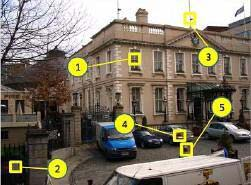
\includegraphics[width=0.8\linewidth]{passpoints.jpg}} % valign=t para alinear la imagen en la parte superior
		\caption{Ejemplo de \textit{Passpoints}. Fuente: \cite{wiedenbeck2005passpoints}}
		\label{passpoints-example}
	\end{minipage}%
	
\end{figure}
En la fase de autenticación el usuario tendrá  que  seleccionar dichos puntos en el mismo orden que en la fase de registro. En  este  sistema  cualquier  imagen  puede  ser  utilizada  (pinturas,  fotos  naturales,  fotos  familiares,  etc),  y  puede  ser seleccionada  por  el  usuario  o proveídas por  el  sistema.  La  imagen  debe  tener  cientos  de  puntos  probables  de  ser seleccionados y deben estar diseminados de forma homogénea para mayor seguridad.
 
Por motivos de seguridad, el sistema  no  almacena  de  forma explícita la contraseña,  sino  un \textit{hash} de la  misma.  Esto  trae  consigo  el  problema de identificar el usuario legítimo, ya que es muy poco probable que se digiten exactamente los mismos puntos durante las fases de registro y autenticación, haciendo que los \textit{hashes} sean diferentes. 
Para solventar este problema es necesario agregar un margen de error para la selección de los puntos, concidos como región de tolerancia. Para lograr esto se utiliza una discretización de la imagen, lo que reduce el espacio de contraseñas y aporta información relevante para  llevar  a  cabo  ataques  de  diccionario \cite{zhu2013security}. Además  permite  la  aparición  de  falsos  positivos  y negativos  en  la autenticación  debido  a  la  forma  de  las  regiones  calculadas  utilizando  la  discretización. 

 Una  discusión  acerca  de  la importancia del mecanismo de discretización en los esquemas de contraseñas gráficas y de los diferentes métodos de discretización conocidos hasta el momento puede verse en \cite{birget2006graphical, chiasson2008centered, bicakci2008optimal, kirovski2007click}. 

Otros aspectos negativos a destacar en este sistema son: 

\begin{itemize}
	\item Algunas regiones en la imagen son más propensas a ser seleccionadas por el usuario para formar su contraseña \cite{mypasswordhere}.
	
	\item Dado que este sistema basa su funcionamiento en la selección de 5 puntos en la imagen, la fase de registro y de autenticación pueden extenderse lo que conlleva a que sean vulnerables ante ataques de tipo \textit{Shoulder-Surfing} \cite{rodriguez2019algoritmo}.
	
	\item Si el conjunto de puntos seleccionados por el usuario no sigue un patrón aleatorio es considerada débil y es susceptible a ataques de diccionarios \cite{rodriguez2019algoritmo}.
\end{itemize}

En varios artículos publicados recientemente \cite{sym13050777, lissetMaster, s22051987, herrera2023comparacion, herrera2023nuevo, herrera2023nuevoregulares, herrera2024new} se proponen \textit{test} para evitar el registro de contraseñas gráficas no aleatorias. Estos resultados unidos a la propuesta en \cite{legon2019nuevo} de un modelo probabilístico capaz de medir el nivel de autenticidad de un usuario, conllevan a un aumento significativo en la seguridad de este sistema y por consiguiente lo convierten en una de las alternativas más prometedoras ante las contraseñas alfanuméricas.

\subsection{¿Por qué usar \textit{Passpoints}?}

La notoria falta de seguridad de las contraseñas alfanuméricas, debido a la contradicción que presentan las mismas \cite{zimmermann2020password}, es una señal de que se requieren opciones más seguras y sencillas de usar. En este escenario, el sistema \textit{Passpoints} se erige como una buena alternativa a las tradicionales contraseñas alfanuméricas. La seguridad de este método de autenticación gráfica reside en su espacio de contraseñas \( Q^L \), donde \( Q \) es el tamaño del alfabeto y \( L \) la longitud de la contraseña \cite{legon2019nuevo}. Mientras que en el caso de las contraseñas alfanuméricas este espacio consiste en la cantidad de cadenas que se pueden formar con un alfabeto específico, en \textit{Passpoints} es la cantidad de combinaciones de puntos (píxeles) de la imagen que se utilice.

En la actualidad, los tamaños de imágenes que se manejan rondan los cientos de miles de píxeles, lo que incrementa aún más el espacio de contraseñas de \textit{Passpoints}. Esto tiene un impacto positivo en su nivel de seguridad y resistencia a ataques de fuerza bruta. Al ser un método novedoso y poco conocido, no existen grandes bases de datos de contraseñas \textit{Passpoints}, a diferencia de la enorme cantidad de información y recopilaciones de contraseñas alfanuméricas disponibles en Internet. Esta falta de información le otorga una mayor resistencia a \textit{Passpoints} ante ataques de diccionario \cite{weakpassw}.

Además, al explotar la capacidad humana de reconocer patrones en imágenes, \textit{Passpoints} facilita el recuerdo de las contraseñas para cualquier tipo de persona, desde niños y adolescentes hasta personas de la tercera edad. Esto contrasta con las contraseñas alfanuméricas, donde, para garantizar la seguridad, se hace necesario que los usuarios memoricen largas cadenas con altos niveles de aleatoriedad. En \cite{rodriguez2018seguridad} se ratifica la posición de \textit{Passpoints} como el método de autenticación gráfica más conveniente, a través de una comparación y evaluación crítica de los diferentes métodos existentes.

\subsection{Región de Tolerancia}
La región de tolerancia \cite{legon2019nuevo, borrego2018debilidades} de un punto \(p\) se define como el conjunto de puntos de la imagen que son aceptados como válidos durante la autenticación para el punto original \(p_0\), y se denota como \(R_T\). Sea \(I\) el conjunto de píxeles de la imagen, y \(f\) una función tal que para todo punto de la imagen devuelve 1 si es aceptado y 0 en caso contrario. Entonces, \(R_T\) quedaría definido como:

\begin{equation}
	R_T = \{p, p \in I \cap f(p) = 1\} \label{eq:region_tolerancia}
\end{equation}

Puede interpretarse la región de tolerancia como el error permitido al usuario en el momento de seleccionar su contraseña.

\subsubsection{Punto \texorpdfstring{$r$}{r}-seguro}
Un punto se considera $r-seguro$ \cite{legon2019nuevo,  borrego2018debilidades} para un radio \(r\) si y solo si todo punto que está a una distancia \(r\) de él se incluye en la región de tolerancia. Sea \(I\) el conjunto de píxeles de una imagen, \(p_0\) un punto de la imagen y \(R_T\) la región de tolerancia. Se dice que \(p_0\) es $r-seguro$ si y solo si:
\begin{equation}
	\forall p \in I: d(p_0, p) < r \Rightarrow p \in R_T \label{eq:r_seguro}
\end{equation}
		
\begin{figure}[h]
			\centering
			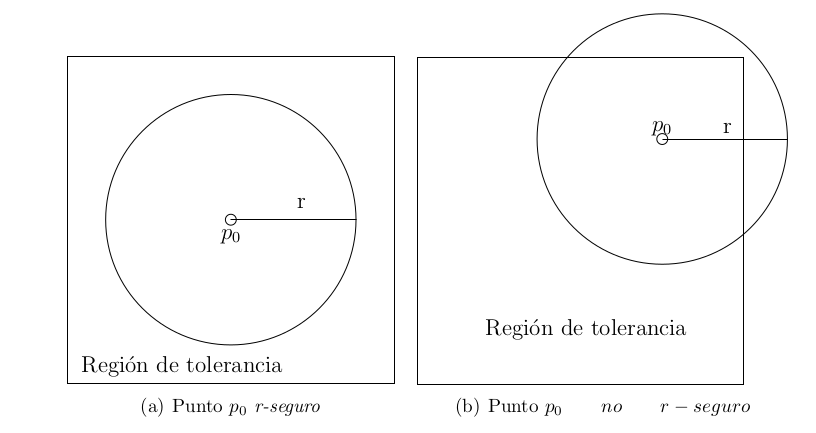
\includegraphics[width=0.5\textwidth]{punto-r-seguro.png}			
			\caption{Ejemplo de punto $r-seguro$ y punto no $r-seguro$. Fuente: \cite{legon2019nuevo} }
		\end{figure}
		
	
\subsection{Problema del Vértice}
Este problema surge durante la fase de registro \cite{  birget2006graphical, legon2019nuevo, borrego2018debilidades}, cuando el usuario puede seleccionar un punto que no es $r-seguro$. Hay dos casos posibles: seleccionar un punto localizado exactamente en los vértices o aristas de la región de la partición, o seleccionar un punto que está situado a una distancia \(d < r\) de los mismos. El primer caso plantea un problema de decisión para determinar la región de tolerancia del punto. Por lo que resulta necesario discretizar las imágenes de tal manera que cada punto pertenezca a una región de tolerancia.

\subsection{Problema del Hash}
Por temas de seguridad, las contraseñas no pueden almacenarse en texto claro. Es necesaria una forma segura de representarlas tal que para cada contraseña exista un identificador único y que estas no sean recuperables desde dicho identificador. Las funciones \textit{hash} \cite{legon2019nuevo, borrego2018debilidades} encajan perfectamente con esta definición, por lo que son un buen recurso a utilizar para almacenar las contraseñas. Sin embargo, usando un \textit{hash} surge la problemática de que cada punto de la región de tolerancia tendrá un \textit{hash} diferente, impidiendo así que guardar el \textit{hash} de los puntos seleccionados sea una buena opción. Utilizando como parámetro de la función \textit{hash} no solo un punto, sino toda su región de tolerancia, no solo se garantiza que se puedan guardar los \textit{hashes} de las contraseñas, sino que también aumenta la cardinalidad del espacio de entrada de la función \textit{hash}, lo que dificulta los ataques de fuerza bruta.
	
\subsection{M\'etodos de Discretizaci\'on}	
Es sencillo percatarse de la baja probabilidad de que un usuario seleccione siempre exactamente el mismo pixel en las fases de registro y autenticación, situación que se agrava aún más en escenarios como el de los teléfonos móviles, cajeros y otras situaciones donde el usuario no posee un puntero digital. Es por  esto que se hace necesario dar un margen de error a cada punto de la contraseña Passpoints, a la región definida por el punto y su margen de error se le conoce como región de tolerancia. Una forma eficiente y segura de introducir esta región de tolerancia en un sistema de autenticación gráfica \textit{Passpoints} es utilizando una discretización.
\subsubsection{Discretización Robusta}

Para evitar el problema del vértice \cite{birget2006graphical}, la discretizaci\'on Robusta utiliza un conjunto de tres particiones diferentes de la imagen. Esto garantiza que cada punto es $r-seguro$ en al menos una de dichas particiones. Esto se logra asegurando una separación de al menos $r$ píxeles entre el punto y el borde de alguna de las tres particiones \cite{zhu2013security, chiasson2008centered}. Se toman cuadrículas de dimensiones \(6r \times 6r\) y cada partición debe estar separada una distancia \(2r\) del resto. Durante la fase de autenticación, debido a la construcción de las particiones, cualquier punto a una distancia \(d \leq r\) del punto original pertenecerá al mismo cuadrante, lo que garantiza la autenticación del usuario ya que la salida de la función \textit{hash} será la misma. Por otro lado, cualquier punto a una distancia mayor a \(5\sqrt{2}r\) pertenecerá a otro cuadrante, lo que garantiza la no autenticación del usuario ilegítimo.

		\begin{figure}[H]
			\centering
			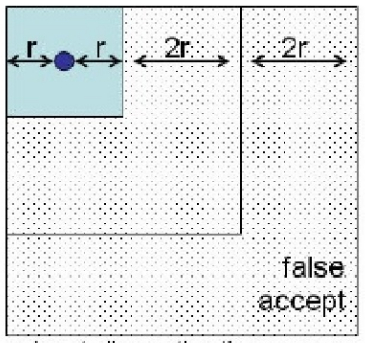
\includegraphics[width=0.25\textwidth]{image4.jpg}
			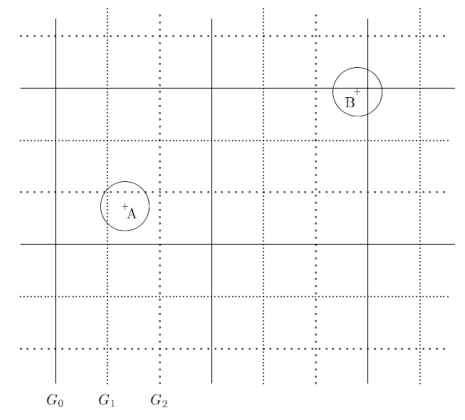
\includegraphics[width=0.27\textwidth]{image2.png}
			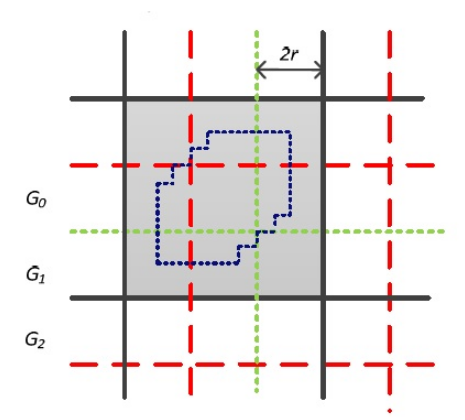
\includegraphics[width=0.28\textwidth]{image3.png}
			\caption{Regiones de la discretizaci\'on Robusta. Fuentes: \cite{zhu2013security} y \cite{chiasson2008centered}.}
		\end{figure}
	
\subsubsection{Discretización Centrada}
	
La Discretización Centrada \cite{chiasson2008centered} ofrece mejoras en usabilidad y seguridad en comparación con la discretización Robusta. Esta técnica garantiza que la región de tolerancia esté centrada en el punto seleccionado para la contraseña, resolviendo así el problema del vértice. Al determinar una región de dimensiones \(2r \times 2r\) centrada en el punto. Este método funciona encontrando, en cada dimensión de la imagen (\textit{x}, \textit{y}), un segmento de longitud \(2r\) en el cual el centro sea el punto originalmente seleccionado en el registro. Sea \textit{x} un punto en la semirrecta numérica que comprende los valores entre 0 y \textit{m}, donde \textit{m} es el ancho o largo de la imagen, dependiendo de la dimensión que se quiera calcular. A partir de ese segmento, se divide el resto del intervalo $[0, m]$ en subintervalos de igual longitud.

En la mayoría de los casos, habrá sobrantes de tamaño \(d\), donde \(d\) pertenece al intervalo $[0, 2r]$, por lo que si se almacena el valor de \(d\) es posible reconstruir la partición realizada comenzando en \(d\), donde uno de estos subintervalos estará centrado en \textit{x}. Una vez establecido el radio \textit{r} y el punto de la contraseña \textit{x}, se puede calcular la región de tolerancia. Se calcula el sobrante \textit{d} que se utilizará luego en la fase de autenticación:
\begin{equation}
	d\equiv(x - r)\mod{2r} \label{eq:sobrante}
\end{equation}

Determinar el intervalo exacto \textit{i} donde se encuentra \textit{x}:
\begin{equation}
	i = \left\lfloor \frac{x - r}{2r} \right\rfloor \label{eq:intervalo_registro}
\end{equation}

Una vez seleccionado el punto $x'$ durante la fase de autenticación, se halla el intervalo $i'$ donde este se encuentra:
\begin{equation}
	i' = \left\lfloor \frac{x' - r}{2r} \right\rfloor \label{eq:intervalo_autenticacion}
\end{equation}
Nótese que \textit{i} no está centrado en $x'$, pero \(|x - x'| < r \rightarrow i = i'\). Por tanto, se utiliza \textit{i} como componente de la contraseña.

	\begin{figure}[H]
		\centering
		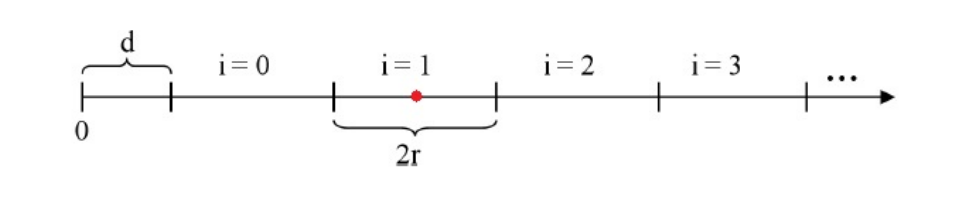
\includegraphics[width=0.9\textwidth]{image5.png}	
		\caption{Ejemplo de recta num\'erica discretizada centralmente. Fuente: \cite{bicakci2008optimal}}	
	\end{figure}

Este método de autenticación supone una mejora sustancial en cuanto a su complejidad de implementación, ya que elimina la necesidad de crear varias particiones en la imagen. Sin embargo, este método introduce un nuevo problema: la necesidad de almacenar el valor \textit{d} en texto claro para poder efectuar la autenticación correctamente. Una posible solución a este problema sería encriptar este valor de forma reversible y almacenarlo junto al \textit{hash} de la contraseña concatenándolo al mismo. Esto permitiría al sistema, durante la fase de autenticación, recuperar estos datos y determinar si los puntos seleccionados son válidos o no.


\subsubsection{Discretización Óptima}
	
Este método mantiene la filosofía de particionar la imagen generando una región centrada en el punto original de la contraseña, pero utiliza propiedades de la aritmética modular para construirla \cite{bicakci2008optimal}. Sean \textit{r} el radio de tolerancia y \textit{X} el punto seleccionado por el usuario, se calcula:
\begin{equation}
	\begin{aligned}
		\textit{X} \mod{2r} \geq r &\rightarrow \phi \equiv X \mod{r} \\
		\textit{X} \mod{2r} < r &\rightarrow \phi \equiv (X \mod{2r}) - r
	\end{aligned}
	\label{eq:phi}
\end{equation}
De forma análoga se calcula:
\begin{equation}
	\begin{aligned}
		\textit{Y} \mod{2r} \geq r &\rightarrow \varphi \equiv Y \mod{r} \\
		\textit{Y} \mod{2r} < r &\rightarrow \varphi \equiv (Y \mod{2r}) - r
	\end{aligned}
	\label{eq:varphi}
\end{equation}
Estos valores (\(\phi\)) y (\(\varphi\)) se almacenan en claro en el sistema junto a los \textit{hashes}:
\begin{equation}
	S_X = \frac{X - \phi}{2r}, \quad S_Y = \frac{Y - \varphi}{2r} \label{eq:hashes}
\end{equation}

Durante la fase de autenticación, el usuario selecciona el píxel ($X'$, $Y'$), utilizando los valores de (\(\phi\)) y (\(\varphi\)) almacenados para ese usuario se calculan los \textit{hashes} \(S_{X'}\) y \(S_{Y'}\) cumpliéndose que se garantiza la autenticación.
\begin{equation}
	\|(X, Y) - (X', Y')\| < r \rightarrow S_{X'} = S_X \land S_{Y'} = S_Y \label{eq:autenticacion}
\end{equation}
Este método es más eficiente que los descritos anteriormente, ya que su implementación a nivel computacional tiene una menor complejidad. Al tomar como base la aritmética modular se reduce la complejidad de los cálculos necesarios. No soluciona el problema del anterior método debido a que mantiene la necesidad de guardar texto claro junto con  las  contraseñas,  en  este  caso  son  los  valores   ($\phi$)  y  ($\varphi$).  Aunque  esto tiene  una  solución  rápida  que comparte con la discretización Centrada.

\subsubsection{Discretización mediante polígonos de Voronoi}
Otras propuestas de discretización encontradas en la bibliografía es la hecha por Kirovski et al. \cite{kirovski2007click}, donde proponen utilizar diagramas de Voronoi. Partiendo de los puntos más probables de ser seleccionados en la imagen (conocidos como \textit{Hotspots} en la literatura), propone aplicar una discretización de Voronoi ponderada usando una heurística para maximizar la entropía \(H(P_w)\), tratando de obtener polígonos equiprobables. Su ventaja principal es que todos los polígonos de la partición obtenida poseen aproximadamente la misma probabilidad a priori de que el usuario escoja un punto de ese polígono. Esta propiedad parece ofrecer mejor resistencia a los ataques de diccionario basados en \textit{Hotspots}. Sin embargo, en \cite{zhu2013securityl} se afirma que la propuesta de \cite{kirovski2007click} sigue dejando información en claro, útil para ataques de diccionario.

\subsubsection{Problemas de los métodos de discretización}
	
El uso de los métodos de discretización conlleva a ciertas limitaciones durante la autenticación. Una de estas es la falta de diferenciación entre los puntos que se encuentran dentro de la región de tolerancia. Todos los puntos reciben el mismo tratamiento, lo cual contradice el comportamiento esperado por parte del usuario legítimo, que debería seleccionar con mayor frecuencia los puntos más cercanos al punto original. Además, al representar la región de tolerancia como un polígono en lugar de un círculo, existe la posibilidad de obtener falsos positivos, es decir, puntos que se encuentran a una distancia mayor que el radio de tolerancia establecido pero que aún se consideran válidos como parte de la contraseña \cite{blonder1996graphical, borrego2018debilidades}. Otro problema se presenta cuando existen puntos situados a la misma distancia del punto seleccionado como parte de la contraseña, siendo ambos válidos para el usuario legítimo. Sin embargo, uno de ellos puede quedar dentro de la región de tolerancia determinada por la discretización y el otro no, lo que genera falsos negativos. Además, al segmentar la imagen en cuadrículas, no se toman todos los puntos que deberían determinar la región de radio \textit{r} alrededor del punto seleccionado como contraseña. Esto puede afectar la experiencia del usuario al utilizar el sistema \cite{bicakci2008optimal, borrego2018debilidades}.

En general, las limitaciones de los métodos de discretización radican en el hecho de que definen la región de tolerancia como un polígono, mientras que la distancia se plantea en términos de un círculo. Además, el criterio utilizado para determinar si un punto es válido o no se basa únicamente en la distancia. Otra debilidad de estos métodos es la necesidad de almacenar información adicional para garantizar la autenticación \cite{borrego2018debilidades}, esto podría ser explotado para aumentar la efectividad de ataques de tipo diccionario. Por lo tanto, es importante abordar en trabajos futuros estas limitaciones y buscar mejoras en los métodos de discretización para lograr una mayor precisión en la autenticación y brindar una mejor experiencia de uso al usuario.




\chapter{Propuesta de una implementación del sistema Passpoints}\label{chapter:proposal}
Como se vio en capítulos anteriores, la autenticación gráfica, específicamente las contraseñas gráficas basadas en \textit{Passpoints}, ofrece una alternativa prometedora a la autenticación tradicional. En el presente capítulo, se propone una implementación de dicho sistema en una aplicación práctica y simple, un blog de notas privado. La elección de este ejemplo se fundamenta en su relevancia como aplicación que requiere un mecanismo de autenticación seguro para proteger la privacidad de los datos almacenados, además de permitir evaluar la escalabilidad del sistema. Esta implementación permitirá validar en un entorno real las ventajas de la autenticación con \textit{Passpoints}, demostrando su viabilidad y seguridad. Asimismo, se desarrollará la API REST (Interfaz de Programación de Aplicaciones, Transferencia de Estado Representacional) necesaria para integrar el sistema de autenticación con el blog de notas, así como la interfaz de usuario que permita la creación y gestión de \textit{Passpoints}.



\section{Regi\'on de tolerancia seleccionada}

Debido a la variabilidad de tamaños de imagen y densidad de píxeles de pantalla, el radio de la región de tolerancia se redefinió como un valor $0 < r < 1$, el cual representa el porcentaje de píxeles de la imagen que abarca dicha región. De este modo, el tamaño en píxeles de la región de tolerancia es variable en función de la imagen, pero constante ante la mirada del usuario. Esta estrategia abre la puerta a futuros trabajos, ofreciendo la posibilidad al usuario de seleccionar el tamaño de la región de tolerancia para su contraseña y simplificando el proceso de prueba de varios tamaños de la región. Tambi\'en ayuda a ajustar la representaci\'on de la regi\'on de tolerancia en distintos tama\~nos de pantalla. Para obtener el valor en píxeles del radio de la región de tolerancia se multiplica $r$ por el mínimo entre el largo y ancho de la imagen, es decir, sea $a$ el alto de la imagen, $b$ el ancho, $d_{pixel} = min(b,a)$.

\section{Método de discretización seleccionado}
Por todo lo explicado anteriormente se seleccion\'o la Discretizaci\'on \'Optima utilizando la variante enunciada en \cite{bicakci2008optimal} con verificaci\'on de \textit{hash} m\'ultiple. Esto funciona introduciendo un error en el c\'alculo de la discretizaci\'on de cada punto y repitiendo el \textit{hash} del punto de forma recursiva $k$ veces, es decir hallar el \textit{hash} de la salida del anterior. Al hacer esto se vuelve la funci\'on \textit{hash} de cada punto m\'as lenta, dando una capa de seguridad extra ante ataques de diccionario. Repetir el c\'alculo de la funci\'on \textit{hash} varias veces, tambi\'en previene que los puntos sean hallados utilizando \textit{rainbow tables}, dando a\'un m\'as seguridad al sistema.
Para introducir este error en el c\'alculo de la discretizaci\'on de cada punto se hace lo siguiente:

Sea 
\[
d((x,y)) : [0,a] \times [0,b] \to \left(\left\lfloor \frac{ x - \phi }{q} \right\rfloor, \left\lfloor \frac{ y - \varphi }{q} \right\rfloor\right)
\]
el valor resultante de discretizar el punto \((x,y)\) para la imagen \(I\). 

Sea \(r\) la región de tolerancia, \(q\) el cuantil o tamaño de las secciones en que se divide la imagen en cada dimensión, y \(\phi\) y \(\varphi\) los \textit{offsets} correspondientes a cada una. Para que el valor de la discretización tenga un error \(0\), es decir, que la división de la imagen en la discretización sea del mismo tamaño que la región de tolerancia, el valor de \(q\) debe ser \(2r\). 

Esto se debe a que el error es:
\[
\pm \left\lfloor \frac{r}{q} \right\rfloor,
\]
por lo que valores de \(q \leq r\) hacen que haya un error \(e \geq 1\).

Luego, durante la fase de verificación de un punto, se verifican el valor del punto y cada error de este. Es decir, sea \(h\) una función \textit{hash} definida como:
\[
h(x, k) = 
\begin{cases} 
	h'(x), & \text{si } k = 0, \\
	h(h'(x), k-1), & \text{si } k > 0,
\end{cases}
\]


Entonces, sean \(x = (a,b)\), el punto originalmente seleccionado por el usuario, y \(x' = (a',b')\), un punto seleccionado durante la autenticación. Se cumple \(d(x) = d(x')\) si \(\exists i \in [-e, e]\) y \(\exists j \in [-e, e]\) tales que:
\[
h(d(x), k) = h(d(x' + (i, j)), k).
\]

En la figura \ref{flujo_discretization} se presenta un diagrama de flujo que refleja el funcionamiento de este proceso.

\begin{figure}[h]
	\centering
	\begin{tikzpicture}[node distance=1.5cm]
		
		% Nodes
		\node (start) [startstop] {Inicio};
		\node (discretize) [process, below of=start] {Discretizar contraseña};
		\node (take_phi_varphi) [io, below of=discretize] {Tomar $\phi$ y $\varphi$ de los puntos originales};
		\node (loop_points) [process, below of=take_phi_varphi] {Iterar sobre los puntos};
		\node (loop_i) [process, below of=loop_points] {Iterar $i \in [-e, e]$};
		\node (loop_j) [process, below of=loop_i] {Iterar $j \in [-e, e]$};
		\node (check_hash) [decision, below of=loop_j] {¿$h(d(x+i, y+j), k) == \text{hash\_original}$?};
		\node (valid) [startstop, right of=check_hash, yshift=2cm, xshift=3cm]  {Contraseña válida};
		\node (invalid) [startstop, below of=check_hash, yshift=-1cm] {Contraseña inválida};
		
		% Arrows
		\draw [arrow] (start) -- (discretize);
		\draw [arrow] (discretize) -- (take_phi_varphi);
		\draw [arrow] (take_phi_varphi) -- (loop_points);
		\draw [arrow] (loop_points) -- (loop_i);
		\draw [arrow] (loop_i) -- (loop_j);
		\draw [arrow] (loop_j) -- (check_hash);
		\draw [arrow] (check_hash.east) -- ++(1,0) -- ++(0,1.5) -- node[anchor=west] {Si} (valid.south);
		\draw [arrow] (check_hash.south) -- node[anchor=west] {termina} (invalid.north);
		
		
		% Loops
		\draw [arrow] (check_hash.west)  -- ++(-1,0)  |- node[above] {No} (loop_j.west);
		\draw [arrow] (loop_j.west) -- ++(-1,0) |- (loop_i.west);
		\draw [arrow] (loop_i.west) -- ++(-1,0) |- (loop_points.west);
		
	\end{tikzpicture}
	\caption{Diagrama de flujo de verificación de contraseña usando la Discretizaci\'on \'Optima}
	\label{flujo_discretization}
\end{figure}

\section{Funcionamiento de la aplicación}


\subsection{Flujo en la API}
Para acceder al sistema, el usuario debe registrarse introduciendo sus credenciales y estableciendo su contraseña utilizando \textit{Passpoints}. Durante el registro, se solicita al usuario que seleccione 5 puntos sobre una imagen, de una lista predeterminada por el sistema. La regi\'on de tolerancia se ver\'a como un recuadro rojo semitransparente centrado en el punto seleccionado por el usuario en la imagen. En el servidor, se calcula la discretización de la imagen y el \textit{hash} de los puntos seleccionados, almacenándose junto con los datos necesarios para la posterior autenticación. Para llevar a cabo la discretización de la imagen, se empleó la Discretización Óptima. Los datos necesarios para la autenticación, como  ($\phi$) y ($\varphi$), son guardados en texto claro para posteriores estudios, pero en una aplicaci\'on real estos deben ser cifrados de forma reversible antes de ser guardados. En la fase de autenticaci\'on el usuario vuelve a seleccionar los 5 puntos anteriormente fijados en la fase de registro, teniendo en cuenta la regi\'on de tolerancia del sistema. Dichos puntos ir\'an a la API en donde se calcular\'a su \textit{hash}, si este coincide con el almacenado por el usuario leg\'itimo se le dar\'a acceso a las notas, en caso contrario se le devuelve un error. Los puntos utilizados para la autenticaci\'on y su estatus de fallido, o no, son almacenados tambi\'en para posteriores estudios. En las figuras \ref{flujo_registro} y \ref{flujo_auth} se pueden ver diagramas de flujo para cada proceso, registro y  autenticaci\'on .

\begin{figure}[H]
	\begin{minipage}[b]{0.42\linewidth}  % Segundo cuadrado, 48% del ancho de línea
		
		\begin{tikzpicture}[node distance=1.5cm]
			
			
			\node (register) [process] {Inicio Registro de usuario};
			
			\node (credentials) [io, below of=register] {Ingresar credenciales};
			
			\node (passpoints) [process, below of=credentials] {Establecer contraseña con \textit{Passpoints}};
			
			\node (select_points) [io, below of=passpoints] {Seleccionar 5 puntos en la imagen};
			
			\node (display_tolerance) [process, below of=select_points] {Mostrar región de tolerancia};
			
		\node (discretize_hash) [process, below of=display_tolerance] 
		{\shortstack{Calcular discretización\\ de la imagen y\\ \textit{hash} de puntos}};
			
			\node (store_data) [process, below of=discretize_hash] {Almacenar datos para autenticación};
			\node (end_register) [startstop, below of=store_data] {Fin de registro};
			
			
			
			
			
			
			\draw [arrow] (register) -- (credentials);
			\draw [arrow] (credentials) -- (passpoints);
			\draw [arrow] (passpoints) -- (select_points);
			\draw [arrow] (select_points) -- (display_tolerance);
			\draw [arrow] (display_tolerance) -- (discretize_hash);
			\draw [arrow] (discretize_hash) -- (store_data);
			\draw [arrow] (store_data) -- (end_register);
			
			
		\end{tikzpicture}
		\caption{Diagrama de flujo registro con \textit{Passpoints}}
			\label{flujo_registro}
	
	\end{minipage} % Espacio vertical entre filas
	\hfill
	\begin{minipage}[b]{0.42\linewidth}  % Segundo cuadrado, 48% del ancho de línea
	
		\begin{tikzpicture}[node distance=1.5cm]
			
			\node (auth_start) [startstop] {Inicio de autenticación};
			
			\node (auth_points) [io, below of=auth_start] {Seleccionar 5 puntos (autenticación)};
			
			\node (auth_process) [process, below of=auth_points] {Calcular \textit{hash} de puntos};
			
			\node (check_hash) [decision, below of=auth_process] {Hash coincide con el almacenado?};
			
			\node (access_granted) [startstop, below of=check_hash, yshift=-0.5cm, xshift=-2.5cm] {Acceso a notas};
			
			\node (access_denied) [startstop, below of=check_hash, yshift=-0.5cm, xshift=2.5cm] {Error de autenticación};
			
			
			
			
			\draw [arrow] (auth_start) -- (auth_points);
			\draw [arrow] (auth_points) -- (auth_process);
			\draw [arrow] (auth_process) -- (check_hash);
			\draw [arrow] (check_hash) -- node[anchor=east] {Si} (access_granted);
			\draw [arrow] (check_hash) -- node[anchor=west] {No} (access_denied);
			
		\end{tikzpicture}
		\caption{Diagrama de flujo autenticación con \textit{Passpoints}}
		\label{flujo_auth}
	\end{minipage}
		
\end{figure}


\subsection{Adaptaci\'on a distintos tama\~nos de pantalla}
Para hacer la aplicaci\'on adaptable a diferentes tama\~nos de pantalla se cambi\'o la forma de tomar los puntos, transform\'andolos a coordenadas de imagen.
Sean $(I_X, I_Y)$ las coordenadas de imagen del punto $p_0$ seleccionado por el usuario, $(S_X, S_Y)$ sus coordenadas de pantalla, $S_W$ el ancho de la ventana, $S_h$ el alto de la ventana, $I_W$ el ancho de la imagen, e $I_h$ el alto de la imagen. Entonces, se calculan las coordenadas de imagen como:

\begin{align*}
	I_X &= \left\lfloor \frac{S_X}{S_W} \cdot I_W \right\rfloor \\
	I_Y &= \left\lfloor \frac{S_Y}{S_h} \cdot I_h \right\rfloor
\end{align*}

Esto garantiza la consistencia en las coordenadas de los puntos en diferentes tamaños de pantalla e imagen.

\section{Validación del sistema propuesto}
Para realizar una validaci\'on de usabilidad de este sistema se pide a los usuarios que den una valoraci\'on de su experiencia, para luego ser evaluadas autom\'aticamente utilizando alg\'un modelo de procesamiento de lenguage como \cite{team2023gemini}. En cuanto a la seguridad se utilizar\'a el ataque de diccionario descrito en \cite{van2010purely}. Este ataque consiste en la creaci\'on de 3 diccionarios de contrase\~nas, los dos primeros utilizando herramientas de procesamiento de im\'agenes, espec\'ificamente segmentaci\'on y detecci\'on de bordes. Otro diccionario generado utilizando el modelo de atenci\'on visual \cite{itti2000saliency}. Para generar el diccionario de ataque, se propone en  \cite{van2010purely} un m\'etodo de clusterizaci\'on de los puntos para reducir la dimensionalidad de los diccionarios y evitar puntos redundantes, funciona haciendo que los puntos que est\'en a una distancia $N$, no necesariamente el radio de la regi\'on de tolerancia, se cuenten como el mismo. Tambi\'en se propone una forma de generar los diccionarios gastando menos recursos computacionales y tiempo, se llega a esto a trav\'es de heur\'isticas para encontrar patrones comunes de los usuarios. 


\chapter{Detalles de Implementación}\label{chapter:implementation}
Este capítulo describe la implementación práctica del modelo teórico propuesto en el capítulo anterior. Se detallan las tecnologías utilizadas, las decisiones de diseño, y los desafíos enfrentados durante el desarrollo.

\section{Contexto Tecnol\'ogico}
Para la implementación de la propuesta, se utilizó el lenguaje \textit{JavaScript} tanto en la interfaz de usuario como en la API. Específicamente, para la API se empleó \textit{Supabase}, un servicio Baas (\textit{Backend} como servicio), que proporciona una base de datos \textit{PostgreSQL} y funciones \textit{serverless} ejecutadas en entornos \textit{JavaScript}. En cuanto a la creación de la interfaz de usuario, se utilizaron tecnologías web comunes como \textit{HTML}, \textit{CSS} y \textit{JavaScript}, todas integradas mediante el \textit{framework} \textit{Vue}. El uso de \textit{Vue} permitió agilizar el desarrollo de sitios web interactivos. 

\section{Arquitectura del Sistema}
El sistema utiliza una arquitectura cliente-servidor desacoplada. El \textit{frontend} (interfaz gr\'afica) cumple con el rol de ser la interfaz de usuario, la l\'ogica de presentaci\'on y gestionar la interacci\'on con el usuario. \textit{Supabase} \cite{supabase} act\'ua como \textit{backend}, cumple con el rol de procesamiento de datos, almacenamiento, autenticaci\'on y l\'ogica de negocio.

\subsection{Patrones y estilos arquitect\'onicos involucrados}
Enfoque \textit{serverless} (sin servidor), esto elimina la necesidad de gestionar un servidor tradicional y la necesidad de tener infraestructura propia. Este enfoque es prove\'ido a trav\'es del uso de \textit{Supabase} \cite{supabase}, esto aumenta la escalabilidad a la vez que reduce los tiempos de desarrollo.

\textit{Single Page Application} (SPA), aplicaci\'on de una sola p\'agina, es un enfoque en el que el navegador carga una sola p\'agina y actualiza el contenido din\'amicamente, esto mejora la reactividad de la web y hace m\'as din\'amica la interacci\'on con el usuario. Se obtiene este enfoque con la utilizaci\'on del \textit{framework} (marco de trabajo) de JavaScript \textit{Vue.js} \cite{vuejs} en el desarrollo de la interfaz gr\'afica, este  da las herramientas necesarias para desarrollar de manera pr\'actica y efectiva aplicaciones completas utilizando la arquitectura mencionada, se puede ver la interfaz gr\'afica en el Anexo No 11. (figuras de \ref{register-screen} a \ref{error-scans}).


\begin{table}[ht]
	\centering
	\caption{Características clave de la arquitectura Vue.js + \textit{Supabase} }
	\label{tab:arquitectura}
	\rowcolors{1}{}{gray!10} % Fondo alternado para filas
	\begin{tabular}{|p{2.1cm}|p{2cm}|p{5cm}|p{5cm}|} % Ajustar anchos según sea necesario
		\hline
		\rowcolor{gray!20} % Color del encabezado
		\textbf{Capa} & \textbf{Tecnología} & \textbf{Responsabilidad} & \textbf{Ejemplo} \\
		\hline
		
		Presentación & Vue.js & 
		Renderizar interfaz de usuario, manejar eventos del usuario, gestión de estado local & 
		Componentes Reactivos, formularios de registro, enrutamiento con Vue Router \\
		\hline
		
		Servicios & \textit{Supabase}  & 
		Proveer servicios backend vía API, gestión de autenticación, ejecutar operaciones CRUD & 
		Autenticación con OAuth, consultas a PostgreSQL, webhooks para notificaciones \\
		\hline
		
		Persistencia & PostgreSQL & 
		Almacenamiento transaccional, garantizar ACID, escalado vertical/horizontal & 
		Tabla de usuarios, registros de actividad, relaciones SQL complejas \\
		\hline
	\end{tabular}
\end{table}


\section{M\'odulos de la aplicaci\'on}

\subsection{Selección de la imagen}
\label{subsec:seleccion-imagen}

En ambas fases (registro y autenticación), el sistema presenta al usuario tres imágenes, ver figura \ref{fig:imagenes-sistema}, en orden aleatorio, de las cuales debe seleccionar aquella asociada a su contraseña. Este mecanismo añade una capa adicional de seguridad al evitar que los usuarios seleccionen siempre la misma imagen por dejadez o por la comodidad de tomar siempre la primera imagen de la lista, evitando as\'i que la selecci\'on de imagen sea predecible. 


\begin{figure}[ht]
	\centering
	\begin{minipage}[b]{0.3\textwidth}
		\centering
		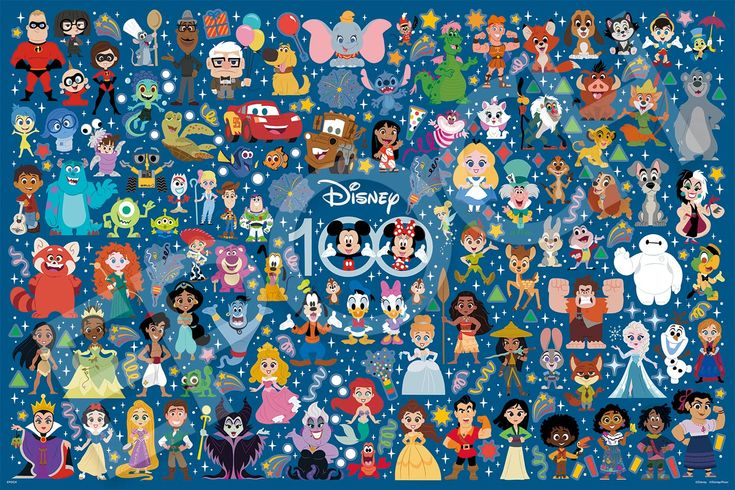
\includegraphics[width=\textwidth]{Graphics/disney.jpeg}
		\caption*{Imagen 1: Disney}
	\end{minipage}
	\hfill
	\begin{minipage}[b]{0.3\textwidth}
		\centering
		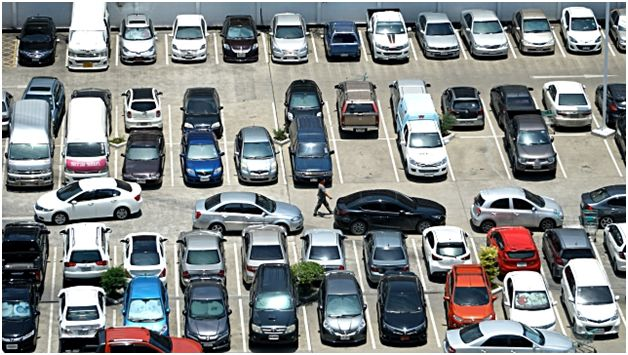
\includegraphics[width=\textwidth]{Graphics/cars.jpeg}
		\caption*{Imagen 3: Cars}
	\end{minipage}
	\hfill
		\begin{minipage}[b]{0.3\textwidth}
		\centering
		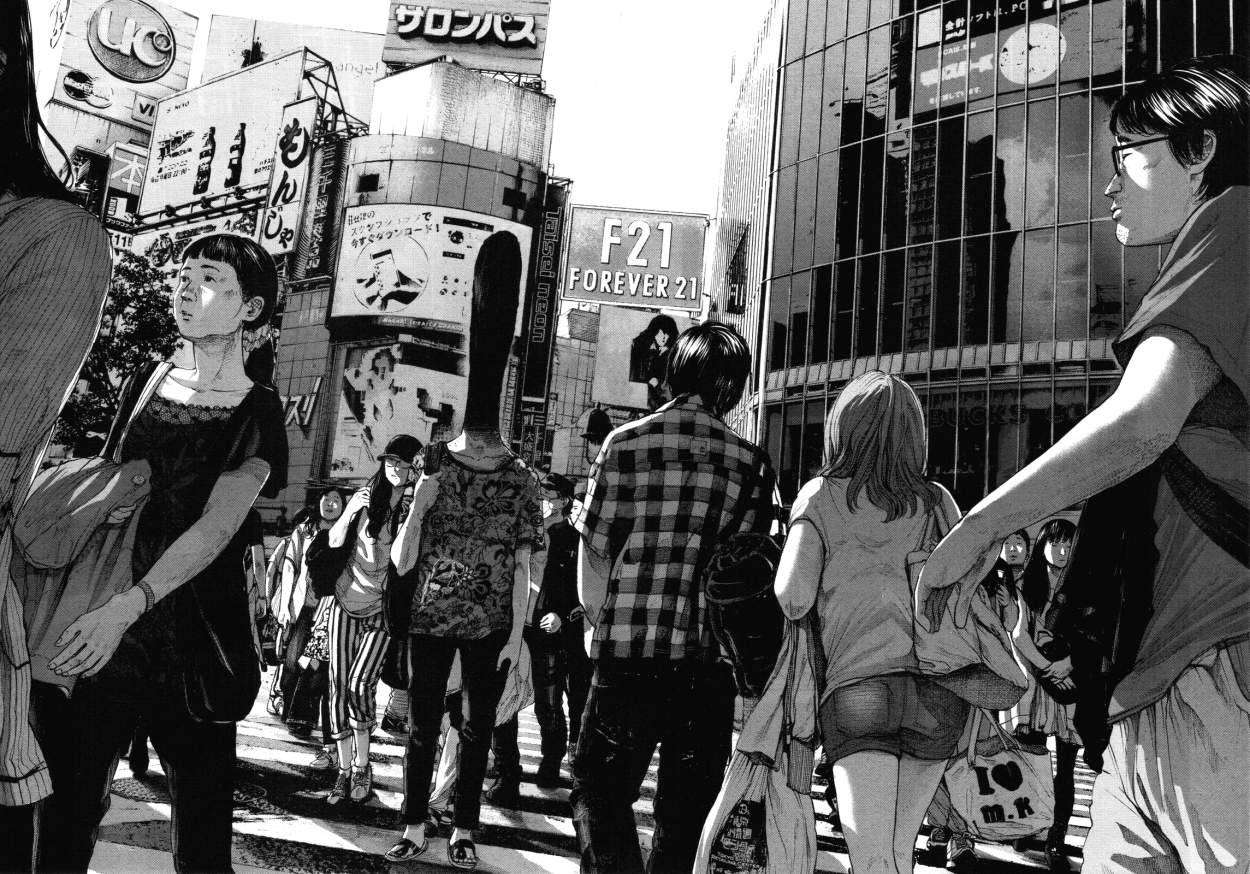
\includegraphics[width=\textwidth]{Graphics/japan.jpg}
		\caption*{Imagen 2: Japan}
	\end{minipage}
	
	\caption{Imágenes disponibles para la selección en el sistema}
	\label{fig:imagenes-sistema}
\end{figure}

La Tabla \ref{tab:uso-imagenes} muestra la distribución real del uso de imágenes según los datos de 33 usuarios. Se observa una preferencia por la imagen Disney (39.39\%), mientras que Japan y Cars presentan una distribución equitativa.


\begin{table}[ht]
	\centering
	\caption{Distribución de uso de imágenes en contraseñas (n = 33)}
	\label{tab:uso-imagenes}
	\begin{tabularx}{0.8\textwidth}{Xcc}
		\toprule
		\textbf{Imagen} & \textbf{Contraseñas} & \textbf{Frecuencia Relativa} \\
		\midrule
		Disney & 13 & 39.39\% \\
		Japan & 10 & 30.30\% \\
		Cars & 10 & 30.30\% \\
		\bottomrule
	\end{tabularx}
	\vspace{0.2cm}

\end{table}

\subsection{Captura de los puntos}
Para seleccionar los puntos se coloca la imagen seleccionada por el usuario de entre un conjunto prove\'ido por el sistema. De esta imagen se obtienen su tama\~no y posici\'on en la pantalla, de tal manera que al reaccionar al evento de \textit{click} del usuario se pueda calcular la regi\'on de la imagen que haya sido seleccionada, esto se puede entender de los ejemplos \ref{point-capture1} y \ref{point-capture2}. 


\begin{lstlisting}[style=mystyle, language=Java, breaklines=true, caption={C\'odigo de selecci\'on de coordenadas de pantalla}, label={point-capture1}, floatplacement=H]
  const { left, top, width, height } =
imagecontainer.value.getBoundingClientRect();
indicators.push({
	x: ((event.clientX - left) / width) * 100,
	y: ((event.clientY - top) / height) * 100,
});
\end{lstlisting}

\begin{lstlisting}[breaklines=true, language=Java, caption={C\'odigo de transformaci\'on en coordenadas de imagen}, label={point-capture2}, floatplacement=H]
	passwordInfo.points = e.map((point: Point) => {
		const { x, y } = point;
		return {
			x: Math.floor((x / 100) * passwordInfo.image.width),
			y: Math.floor((y / 100) * passwordInfo.image.height),
		};
		});
\end{lstlisting}

\subsection{Registro y autenticaci\'on}
\subsubsection{Proceso de Registro}
Durante la fase de registro, el usuario debe ingresar en dos ocasiones su contraseña gráfica (\textit{Passpoints}), ver Anexo No 11. (figuras \ref{register-screen},  \ref{screen-shapes-variety},\ref{error-scans}). Este mecanismo de doble verificación busca incrementar la memorabilidad de la secuencia de \textit{clicks}. Posteriormente, el sistema realiza una llamada a una \textit{edge function} de \textit{Supabase} , a la cual se transmiten:

\begin{itemize}
	\item Correo insertado por el usuario
	\item Nombre de usuario digitado
	\item Identificador de la imagen seleccionada
	\item Tolerancia utilizada 
	\item Ancho y alto de la imagen
	\item Coordenadas $(x,y)$ de los puntos seleccionados
\end{itemize}

Esta función se encarga de: 
\begin{enumerate}
	\item Discretizar la imagen, obteniendo los parámetros $\phi$  y $\varphi$ de cada punto.
	\item Generar el \textit{hash} de ambas instancias de la contraseña (original y de confirmación) utilizando el m\'etodo explicado en el cap\'itulo anterior.
	\item Validar la congruencia entre ambos \textit{hashes}.
	\item Utilizar los m\'odulos prove\'idos por \textit{Supabase}  para el registro y autenticaci\'on del usuario usando esta informaci\'on.
\end{enumerate}

Al proceso de \textit{hashing} se le agrega un n\'umero generado aleatoriamente criptogr\'aficamente seguro. Esto hace que los \textit{hashes} de contrase\~nas iguales sean diferentes y previene ataques de tipo \textit{Rainbow Tables}.

\subsubsection{Mecanismo de registro y autenticaci\'on}
El módulo de autenticación de \textit{Supabase}  emplea un esquema basado en \textit{JSON Web Tokens (JWT)} para:
\begin{itemize}
	\item Gestionar sesiones de usuario
	\item Verificar identidades en cada solicitud
	\item Mantener integridad en la comunicación cliente-servidor
\end{itemize}

Para integrar el sistema \textit{Passpoints} con este servicio:
\begin{itemize}
	\item Se utiliza el \textit{hash} generado del \textit{Passpoints} como contraseña textual en el registro y autenticaci\'on con \textit{Supabase} .
	\item Se preserva el requisito de entrada válida de \textit{Passpoints} para autenticaciones futuras.
	\item Se garantiza compatibilidad con el flujo estándar de OAuth 2.0, lo cual garantiza que se puedan seguir usando los servicios prove\'idos por \textit{Supabase} \cite{supabase}.
\end{itemize}


\begin{table}[ht]
	\centering
	\caption{Estructura de la tabla de usuarios}
	\label{tab:bd-esquema}
	\begin{tabularx}{\textwidth}{lX}
		\toprule
		\textbf{Tabla \texttt{user}} & \textbf{Descripción} \\
		\midrule
		\texttt{id} & Identificador único del usuario (UUID v4) \\
		\texttt{email} & Correo electrónico del usuario (único, formato validado) \\
		\texttt{password\_hash} & Hash de la contraseña gráfica \\
		\texttt{phi\_params} & Parámetros de cuantización espacial (JSON) \\
		\texttt{varphi\_params} & Parámetros de tolerancia (JSON) \\
		\texttt{salt} & Valor aleatorio criptográfico (256 bits) \\
		\texttt{tolerance\_radius} & Radio de tolerancia en píxeles (entero 8-32) \\
	
		\bottomrule
	\end{tabularx}
\end{table}


\begin{table}[ht]
	\centering
	\begin{tabularx}{\textwidth}{lX}
		\toprule
		\textbf{Tabla \texttt{Passwords}} & \textbf{Descripción} \\
		\midrule
		\texttt{user\_id} & Clave foránea a \texttt{user.id} \\
		\texttt{image\_id} & Identificador de la imagen base \\
		\texttt{tolerance} & Radio de tolerancia en píxeles \\
		\texttt{points} & Coordenadas $(x,y)$ en texto claro \\
		\texttt{discretization\_params} & $\phi$ y $\varphi$ en texto claro por cada punto (JSON) \\
		\bottomrule
	\end{tabularx}
\end{table}

\subsubsection{Nota de Seguridad}
La decisión de almacenar en texto claro:
\begin{itemize}
	\item Coordenadas de los puntos.
	\item Parámetros $\phi$ y $\varphi$.
	\item Informaci\'on de la imagen, identificador, ancho, alto.
\end{itemize}

Se restringe exclusivamente a fines académicos. En un entorno productivo se aplicarían las siguientes medidas:
\begin{itemize}
	\item Cifrado AES-256 de todos los parámetros sensibles.
	\item No se guardar\'ian las coordenadas originales de la contrase\~na.
	\item No se guardar\'ia la informaci\'on de la imagen utilizada.
\end{itemize}

\subsection{Flujo de Autenticación}
Durante la fase de autenticación, el usuario debe:

\begin{enumerate}
	\item Seleccionar la imagen utilizada durante el registro de entre tres opciones presentadas en orden aleatorio.
	\item Ingresar su contraseña gráfica (\textit{Passpoints
}) sobre la imagen seleccionada
\end{enumerate}

Este diseño incrementa la conciencia del usuario sobre su elección y reduce la predictibilidad del sistema ante posibles ataques.

\subsubsection{Mecanismos de Seguridad}
El sistema implementa las siguientes protecciones:

\begin{itemize}
	\item Ocultamiento de regiones de tolerancia: Los indicadores visuales (recuadros rojos del tama\~no de la regi\'on de tolerancia) se deshabilitan por defecto para prevenir ataques \textit{shoulder surfing}, aunque el usuario puede habilitarlos.
	\item \textit{Edge function} especializada: Valida las credenciales mediante el flujo:
	\begin{enumerate}
		\item Verificación de existencia del usuario en la base de datos.
		\item Recuperación de parámetros almacenados ($\varphi$, valor aleatorio $salt$, tolerancia $tolerance$, y \textit{hash} original), valores de la tabla \ref{tab:bd-esquema}
		\item Recomputación del \textit{hash} usando el método de discretización descrito en el Capítulo anterior.
		\item Verificaci\'on de la autenticidad de la contrase\~na usando el m\'odulo de autenticaci\'on de \textit{Supabase}.
	\end{enumerate}
\end{itemize}

\begin{table}[ht]
	\centering
	\caption{Parámetros de verificación en autenticación}
	\label{tab:parametros-verificacion}
	\begin{tabularx}{\textwidth}{lXl}
		\toprule
		\textbf{Parámetro} & \textbf{Descripción} & \textbf{Tipo} \\
		\midrule
		$\varphi$ & Lista de $\phi$, $\varphi$ de los puntos & JSON \\
		$c$ & Valor aleatorio  (\textit{salt}) & CHAR (256) \\
		$t$ & Radio de tolerancia & Entero 32 bits \\
		$h$ & \textit{Hash} & \texttt{CHAR(60)} \\
		\bottomrule
	\end{tabularx}
\end{table}

\subsubsection{Gestión de Sesiones}
El servicio de autenticación de \textit{Supabase}  emplea \textit{JSON Web Tokens (JWT)} para:

\begin{itemize}
	\item Generar credenciales temporales con expiración.
	\item Gestionar la validez de los \textit{tokens} en cada petici\'on y restringir acceso a los servicios en funci\'on de las pol\'iticas de seguridad definidas.
	\item Almacenar el estado de sesión en \textit{cookies} HttpOnly/Secure de lado del usuario, a trav\'es de uso de su cliente de JavaScript en la interfaz.
\end{itemize}

La validación resulta en:
\begin{itemize}
	\item Creación de sesión con \textit{token} de acceso/refresh en caso de ser exitosa.
	\item Entrada de un registro en la tabla \textit{auth-passwords} donde se guardan los puntos usados en el intento de autenticaci\'on y el resultado del mismo.
	\item Entrega al cliente de credenciales y datos de sesi\'on para acceder a su informaci\'on en el sistema.
\end{itemize}


\chapter{Validaci\'on del sistema propuesto}\label{chapter:validation}


\section{Análisis del Espacio de Contraseñas con Discretización Óptima}
\label{subsec:espacio-contrasenas}

El espacio de contraseñas resultante para el sistema \textit{Passpoints} utilizando discretización óptima se calcula mediante la ecuación propuesta en \cite{birget2006graphical}:

\begin{equation}
	P = \left( \frac{a}{6r} \cdot \frac{b}{6r} \right)^c
	\label{eq:espacio-contrasenas}
\end{equation}

donde los parámetros se definen como:

\begin{table}[ht]
	\centering
	\caption{Parámetros del espacio de contraseñas}
	\label{tab:parametros-espacio}
	\begin{tabularx}{0.9\textwidth}{lXl}
		\toprule
		\textbf{Símbolo} & \textbf{Descripción} & \textbf{Dominio} \\
		\midrule
		$a \times b$ & Dimensiones de la imagen (en píxeles) & $\mathbb{Z}^+ \times \mathbb{Z}^+$ \\
		$c$ & Cantidad de puntos seleccionados & $c \geq 5$ \\
		$r$ & Radio de la región de tolerancia & $r \in [8, 32]$ \\
		\bottomrule
	\end{tabularx}
\end{table}

\vspace{0.5cm}

Esta formulación establece que el espacio de contraseñas efectivo $P$ crece exponencialmente con respecto a:
\begin{itemize}
	\item La relación $\frac{a \cdot b}{(6r)^2}$: Densidad de puntos discretizados por área
	\item El número de puntos $c$: Complejidad combinatoria de la secuencia
\end{itemize}

Para una imagen típica de $1024 \times 768$ píxeles con parámetros $r = 16$ y $c = 5$:

\begin{align*}
	P &= \left( \frac{1024}{6 \cdot 16} \cdot \frac{768}{6 \cdot 16} \right)^5 \\
	&= \left( \frac{1024}{96} \cdot \frac{768}{96} \right)^5 \\
	&= (10.6667 \times 8.0)^5 \\
	&= (85.3333)^5 \\
	&\approx 4.43 \times 10^9 \text{ combinaciones}
\end{align*}

Este resultado demuestra que incluso con discretización espacial, el sistema mantiene un espacio de contraseñas comparable al de contraseñas textuales complejas ($\sim$10 bits de entropía por punto). Lo que hace inviable un ataque de fuerza bruta.


\section{Ataque a Passpoints}
Para llevar a cabo una validaci\'on de seguridad del sistema, se presenta un ataque de diccionario extra\'ido de \cite{van2010purely}. El ataque consiste en generar 3 diccionarios basados en diferentes criterios. Una vez generados, se lleva a cabo la ejecuci\'on del ataque al sistema.

\subsubsection{Diccionario de ataque basado en detecci\'on de bordes}
Para la detección de bordes, se empleó el algoritmo de Harris \cite{Harris1988ACC}, el cual fue aplicado de manera sistemática a todas las imágenes del sistema. La elección de este método se sustenta en lo expuesto por \cite{van2010purely}, quienes justifican el uso de técnicas de detección de esquinas basándose en la premisa de que los usuarios tienden a seleccionar puntos que coinciden con focos de atención visual. Para identificar dichos puntos, es necesario localizar regiones de mayor contraste en relación con el resto de la imagen, siendo los bordes un ejemplo paradigmático de estas características. Los resultados obtenidos tras la aplicación de este enfoque se presentan en la figura \ref{fig:images-borders }.

\begin{figure}[ht]
	\centering
	\begin{minipage}[hb]{0.3\textwidth}
		\centering
		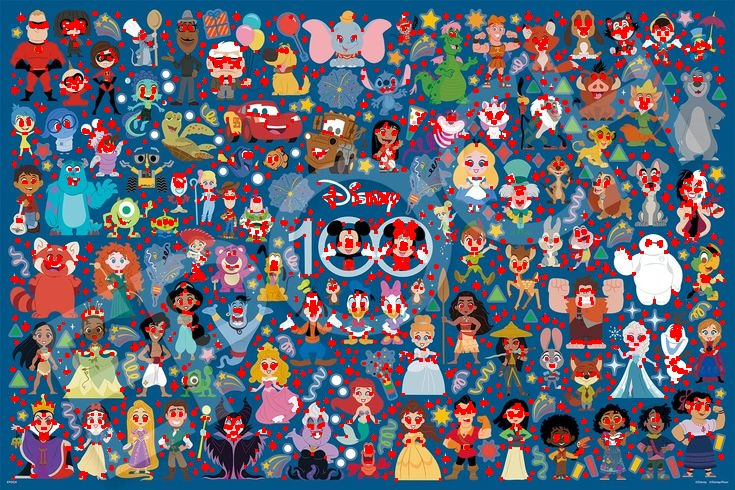
\includegraphics[width=\textwidth]{Graphics/bordes_disney.jpg}
		\captionof*{figure}{Bordes Disney}
	\end{minipage}
	\hfill
	\begin{minipage}[hb]{0.3\textwidth}
		\centering
		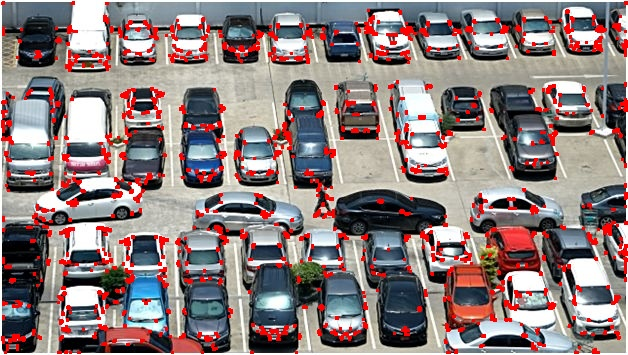
\includegraphics[width=\textwidth]{Graphics/bordes_cars.jpg}
		\captionof*{figure}{Bordes Cars}
	\end{minipage}
	\hfill
	\begin{minipage}[hb]{0.3\textwidth}
		\centering
		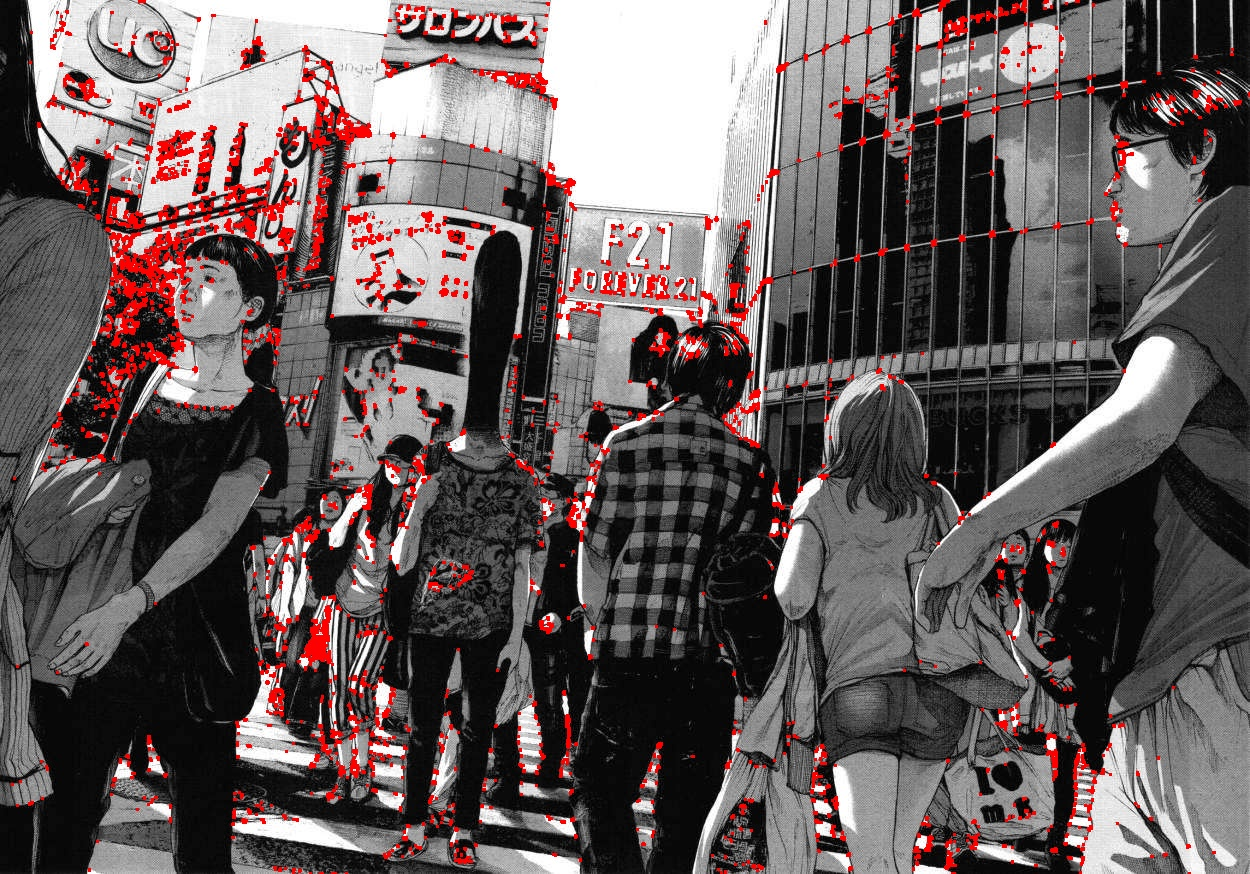
\includegraphics[width=\textwidth]{Graphics/bordes_japan.jpg}
		\captionof*{figure}{Bordes Japan}
	\end{minipage}
	\caption{Imágenes del Sistema con bordes marcados}
	\label{fig:images-borders}
\end{figure}


\subsubsection{Diccionario de ataque basado en segmentaci\'on}
Para la construcción del diccionario de ataque basado en segmentación, se procedió a segmentar las imágenes y determinar sus centros mediante la aplicación del algoritmo \textit{Mean Shift} \cite{Comaniciu2002MeanSA}. A partir de cada segmento obtenido, se utilizó su centro como referencia para generar el diccionario, asegurando que este incorporara la información estructural derivada de la división de cada imagen en sus respectivas regiones. Los resultados de este proceso se muestran en la figura \ref{fig:images-segments }.

\begin{figure}[H]
	\centering
	\begin{minipage}[hb]{0.3\textwidth}
		\centering
		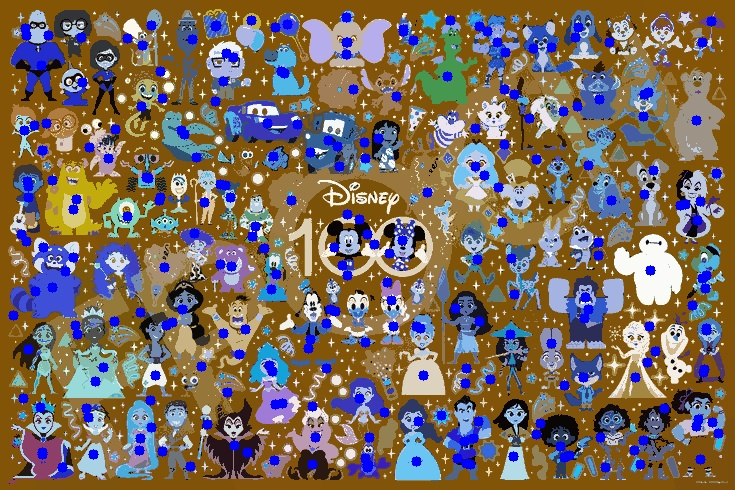
\includegraphics[width=\textwidth]{Graphics/disney-segmented.jpg}
		\captionof*{figure}{Mapa de Segmentaci\'on en imagen Disney}
	\end{minipage}
	\hfill
	\begin{minipage}[hb]{0.3\textwidth}
		\centering
		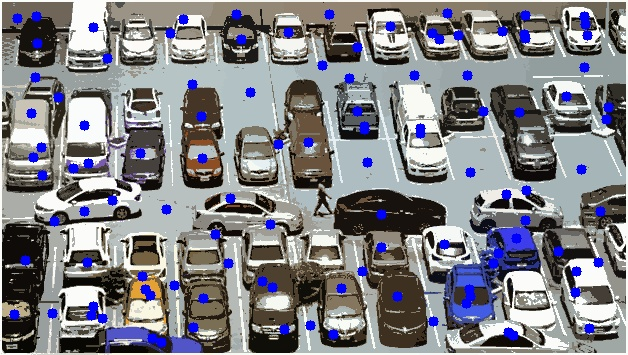
\includegraphics[width=\textwidth]{Graphics/cars-segmented.jpg}
		\captionof*{figure}{Mapa de  segmentaci\'on en imagen Cars}
	\end{minipage}
	\hfill
	\begin{minipage}[hb]{0.3\textwidth}
		\centering
		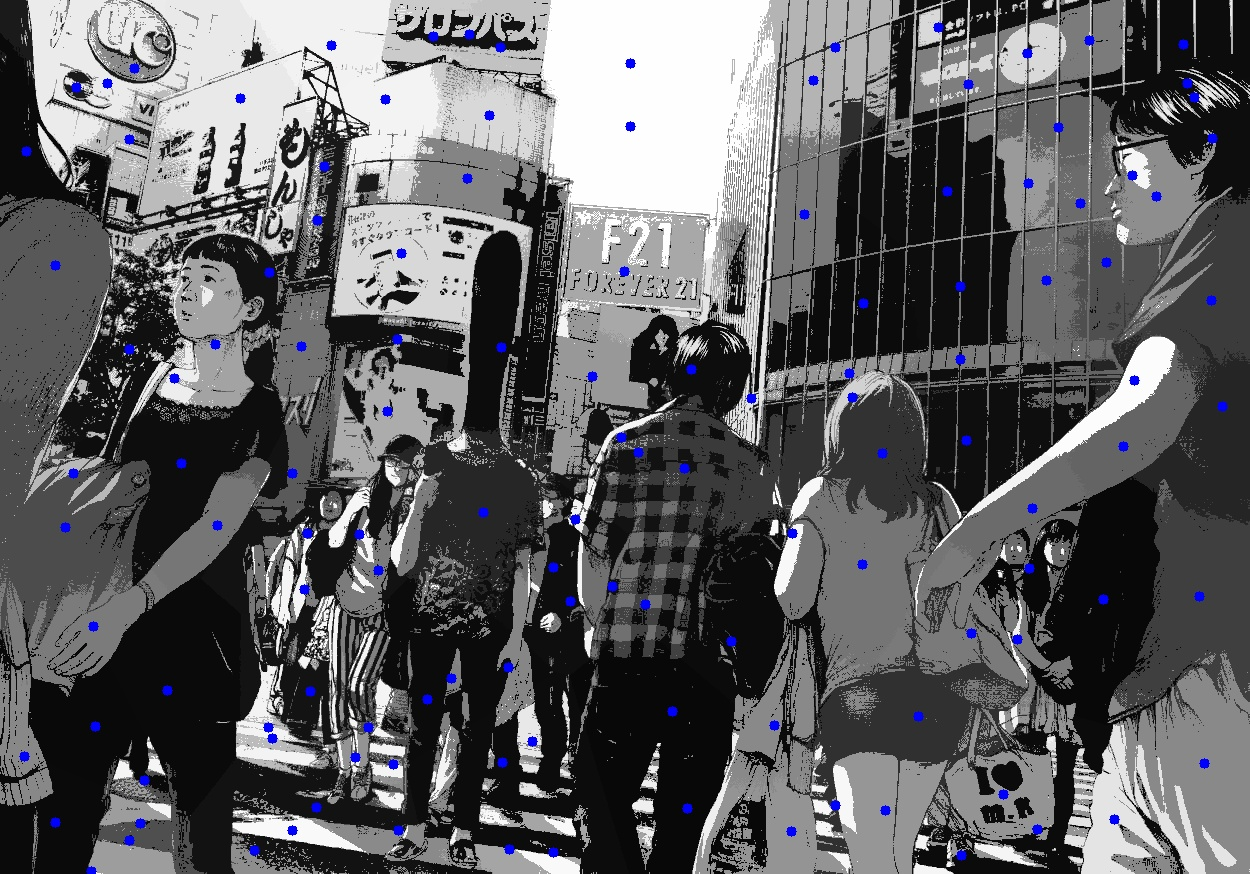
\includegraphics[width=\textwidth]{Graphics/japan-segmented.jpg}
		\captionof*{figure}{Mapa de Segmentaci\'on en imagen Japan}
	\end{minipage}
	\caption{Imágenes del Sistema con sus mapas de segmentaci\'on respectivos y los centros de los mismos marcados}
	\label{fig:images-segments}
\end{figure}

\subsubsection{Diccionario de ataque basado en mapas de atenci\'on visual}
Con el fin de construir el diccionario basado en mapas de atención visual, se calcularon los conjuntos de  puntos m\'as probables a ser seleccionados por los usuarios utilizando un modelo de saliencia visual, el cual modela la forma en que los usuarios miran las im\'agenes. El modelo es el propuesto en \cite{itti2000saliency}, es un modelo \textit{bottom-up}, y se basa en caracter\'isticas como el color, direcci\'on que indica cada pixel y su posici\'on en la imagen. Luego de hallar estos mapas se filtraron sus puntos para determinar los de mayor saliencia visual. Estos fueron utilizados posteriormente en la generaci\'on del diccionario de ataque. Se puede visualizar los puntos seleccionados en las figuras \ref{fig:saliency-map} y \ref{fig:selected-points}.

\begin{figure}[H]
	\centering
	\begin{minipage}[hb]{0.3\textwidth}
		\centering
		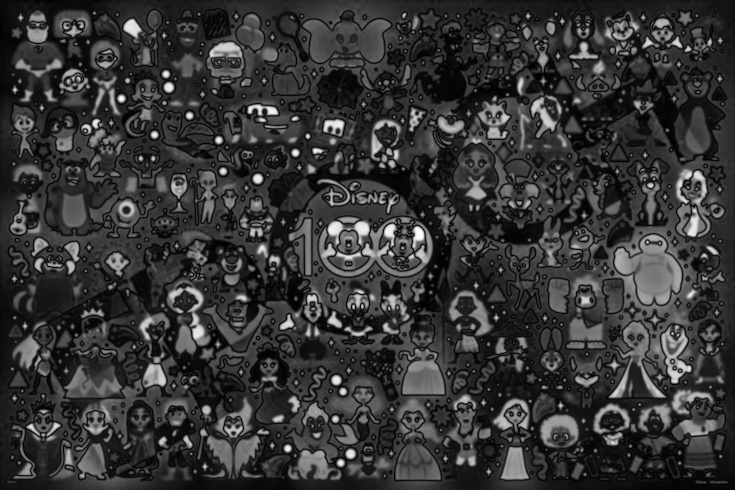
\includegraphics[width=\textwidth]{Graphics/disney-saliency.jpg}
		\captionof*{figure}{Mapa de Atenci\'on en imagen Disney}
	\end{minipage}
	\hfill
	\begin{minipage}[hb]{0.3\textwidth}
		\centering
		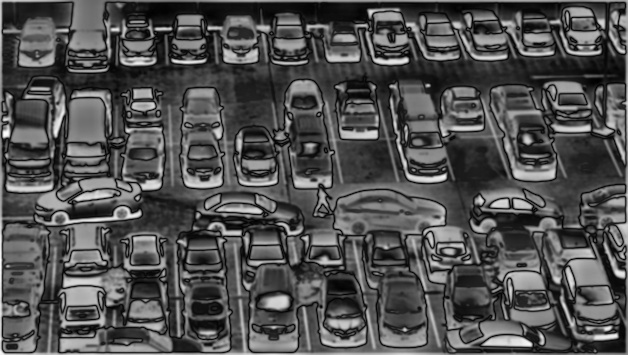
\includegraphics[width=\textwidth]{Graphics/cars-saliency.jpg}
		\captionof*{figure}{Mapa de  Atenci\'on en imagen Cars}
	\end{minipage}
	\hfill
	\begin{minipage}[hb]{0.3\textwidth}
		\centering
		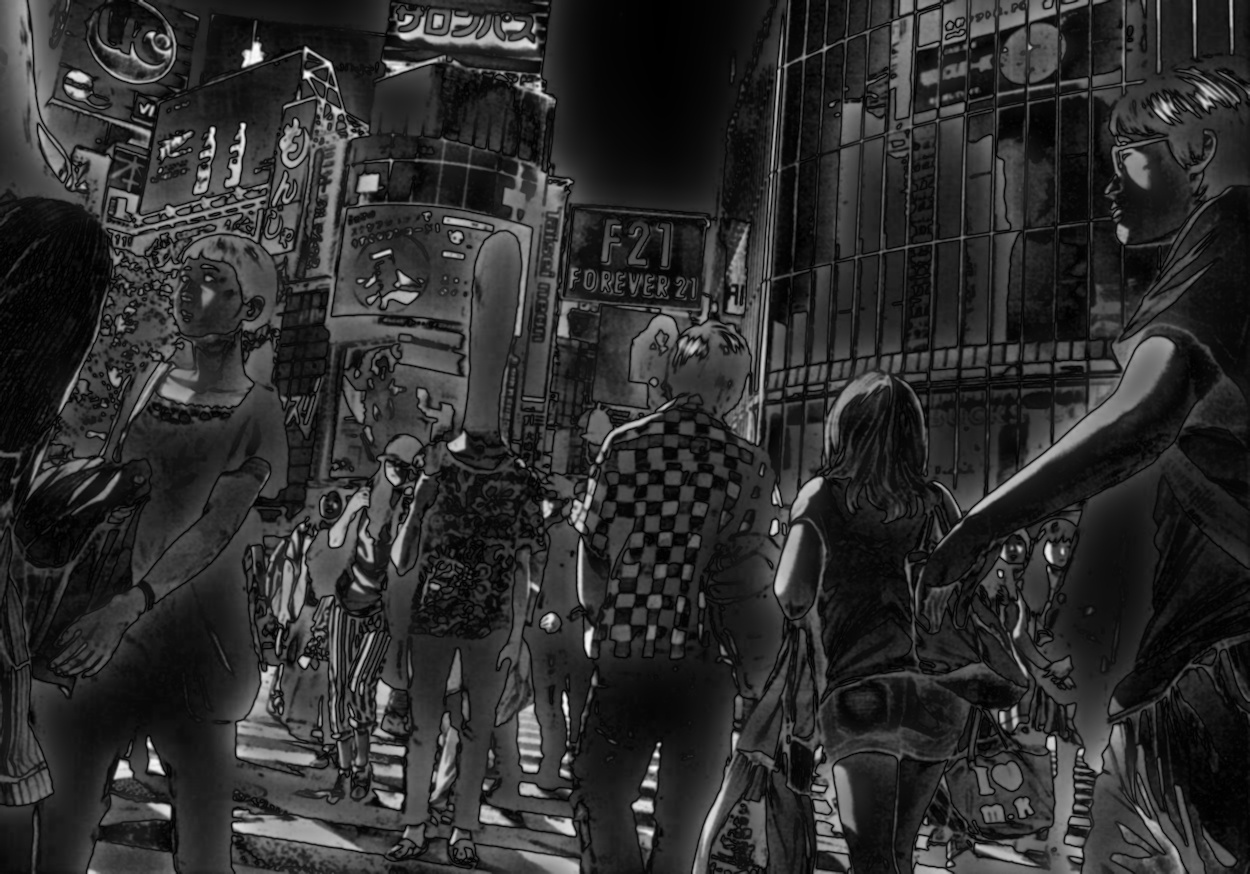
\includegraphics[width=\textwidth]{Graphics/japan-saliency.jpg}
		\captionof*{figure}{Mapa de Atenci\'on en imagen Japan}
	\end{minipage}
	\caption{Imágenes del Sistema con sus mapas de atenci\'on respectivos }
	\label{fig:saliency-map}
\end{figure}

\begin{figure}[H]
	\centering
	\begin{minipage}[hb]{0.3\textwidth}
		\centering
		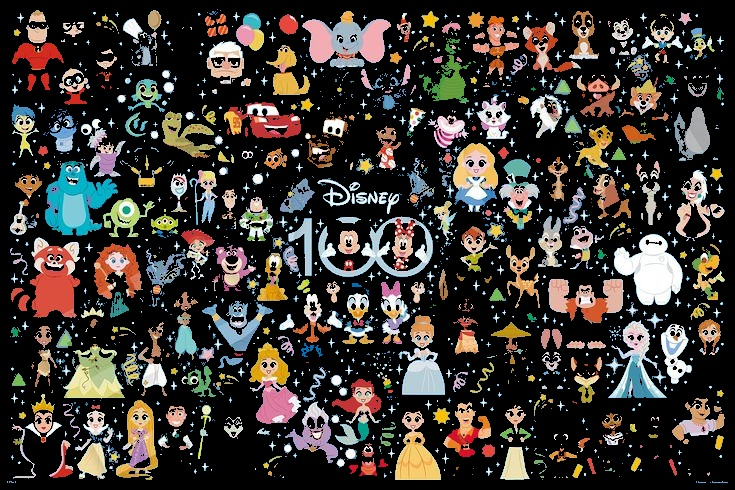
\includegraphics[width=\textwidth]{Graphics/disney-selected-regions.jpg}
		\captionof*{figure}{Regiones seleccionadas en imagen Disney}
	\end{minipage}
	\hfill
	\begin{minipage}[hb]{0.3\textwidth}
		\centering
		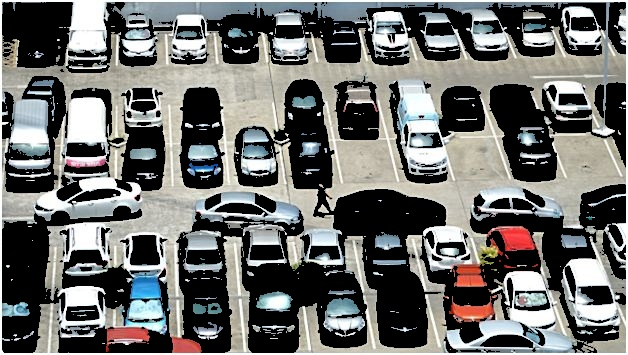
\includegraphics[width=\textwidth]{Graphics/cars-selected-regions.jpg}
		\captionof*{figure}{Regiones seleccionadas en imagen Cars}
	\end{minipage}
	\hfill
	\begin{minipage}[hb]{0.3\textwidth}
		\centering
		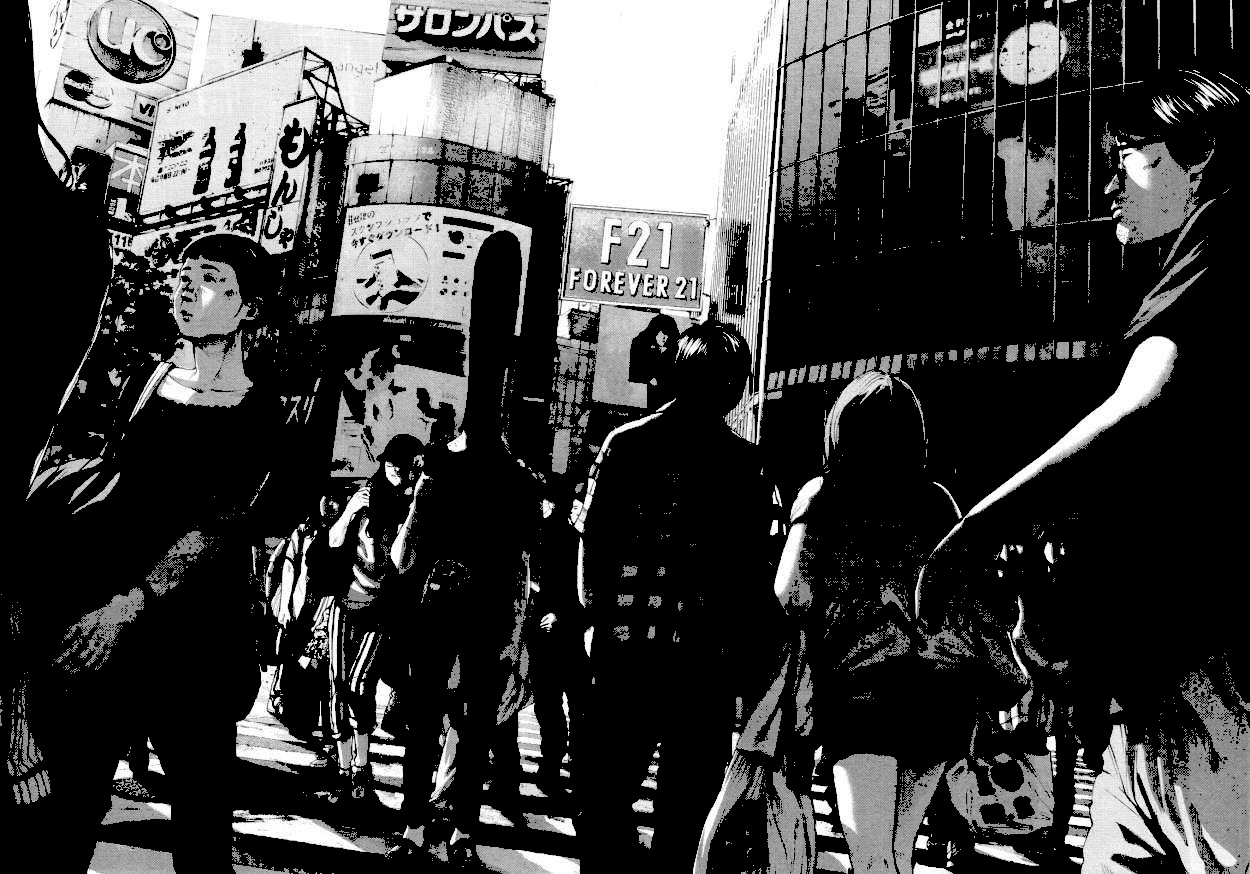
\includegraphics[width=\textwidth]{Graphics/japan-selected-regions.jpg}
		\captionof*{figure}{Regiones seleccionadas en imagen Japan}
	\end{minipage}
	\caption{Imágenes del Sistema con sus respectivas regiones seleccionadas para la creaci\'on del diccionario de ataque}
	\label{fig:selected-points}
\end{figure}


\subsection{Clusterizaci\'on de los puntos }
Para eliminar los puntos que est\'en suficientemente cercanos para caer en la misma regi\'on de tolerancia y reducir las dimensiones de los diccionarios de ataque finales generados, se utiliza el algoritmo de clusterizaci\'on de ventana propuesto en \cite{van2010purely}. Este toma los puntos pertenecientes a una ventana de tama\~no fijo y los sustituye por el pixel del centro geom\'etrico de la ventana. Esto permite eliminar puntos innecesarios y reducir la dimensi\'on del espacio de puntos a analizar para generar un diccionario de ataque final. Para estos fines se tom\'o como tama\~no de ventana $3*r$, donde r es el radio de tolerancia de la imagen en p\'ixeles, dando un margen mayor al generado por la regi\'on original que ser\'ia de $2*r$. Esto permiti\'o reducir la cantidad de puntos a analizar, sin perder mucha informaci\'on. En la tabla \ref{points:void} se puede ver la cantidad de puntos extra\'idos de cada imagen utilizando las t\'ecnicas de procesamiento anteriormente enunciadas. En la tabla \ref{points:cluster} se puede observar la reducci\'on sustancial de la cantidad de puntos despu\'es de aplicar el clusterizado de ventana.
\begin{table}[H]
	\centering
	\caption{Puntos Obtenidos sin clusterizar}
	\label{points:void}
	\begin{tabular}{|l|l|l|l|l|l|l|l|l|l|}
		\hline
		\textbf{im\'agenes/puntos} & \textbf{segmentos } & \textbf{esquinas} & \textbf{saliencia}
		\\ \hline
		\textbf{disney} & 249 & 30 785 & 92 981 \\ \hline
		\textbf{cars} & 110 & 17 826 & 39 764 \\ \hline
		\textbf{japan} & 126 & 47 415 & 203 804  \\ \hline
	
	\end{tabular}
\end{table}

\begin{table}[H]
	\centering
	\caption{Puntos Obtenidos despu\'es de clusterizar}
		\label{points:cluster}
	\begin{tabular}{|l|l|l|l|l|l|l|l|l|l|}
		\hline
		\textbf{im\'agenes/puntos} & \textbf{segmentos} & \textbf{esquinas} & \textbf{saliencia }  \\ \hline
		\textbf{disney} & 36 & 103 & 65  \\ \hline
		\textbf{cars} & 26 & 98 & 38  \\ \hline
		\textbf{japan} & 30 & 82 & 64 \\ \hline
	\end{tabular}
\end{table}

\section{Diccionario de ataque basado en los patrones DIAG y LINE}
Para obtener los diccionarios de ataque que se utiliz\'o el algoritmo basado en grafos propuesto en \cite{van2010purely}. Dicho algoritmo utiliza heur\'isticas para generar contrase\~nas no aleatorias que sigan los patrones DIAG y LINE \cite{s22051987},  comunmente seleccionadas por los usuarios. Para esto se precomputa una matriz de adyacencia M donde para los pares de puntos $i,j \in A$, donde $A$ es un alfabeto de puntos, se cumple.
\[
 M[i,j] = 
\begin{cases} 
	1 & \text{si } (i, j) \in \text{Patrón DIAG o LINE} \\
	0 & \text{si no}
\end{cases}
, \quad \text{para } i,j \in A
\] 

En el caso de la generaci\'on de los grafos utilizados en este ataque se utiliz\'o el par\'ametro de $\tau=9$ que da patrones de relajaci\'on normales, seg\'un \cite{van2010purely} y la distancia m\'axima entre puntos ($Td = \infty$), lo que genera patrones m\'as ce\~nidos a la heur\'istica, en la Tabla \ref{graphs},  se observan los grafos generados para estas im\'agenes con los par\'ametros anteriormente enunciados y el patr\'on DIAG.



\begin{table}[H]
	\centering
	\begin{tabular}{|c|c|c|c|}
		\hline
		& Disney & Cars & Japan \\ \hline
		Segmentos & 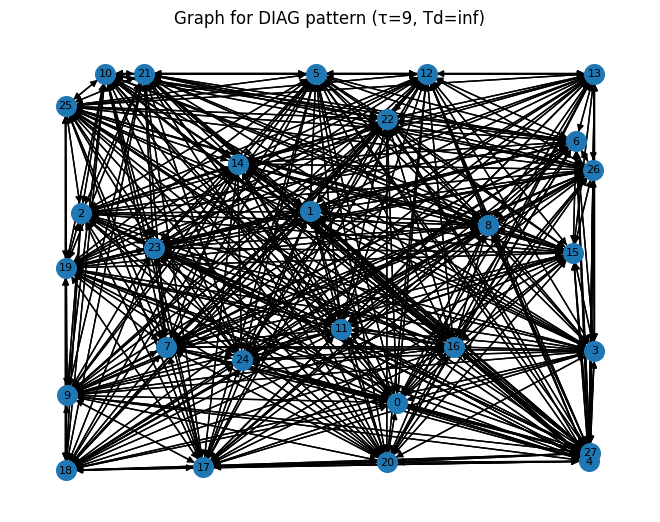
\includegraphics[width=3.5cm]{Graphics/disney-cluster-graph.png} 
		& 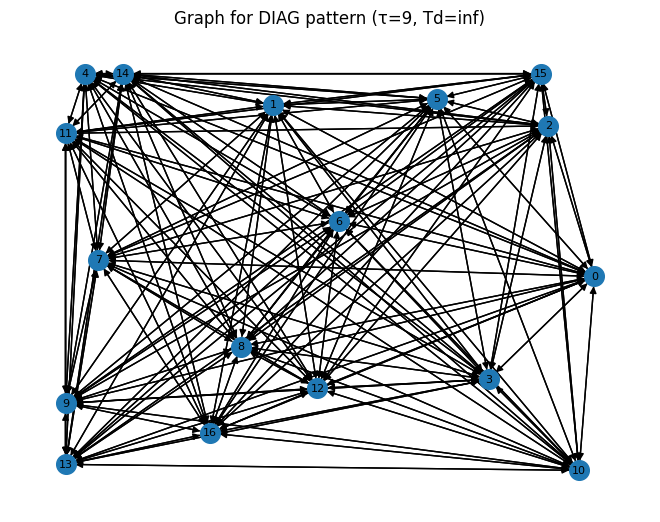
\includegraphics[width=3.5cm]{Graphics/cars-cluster-graph.png} 
		& 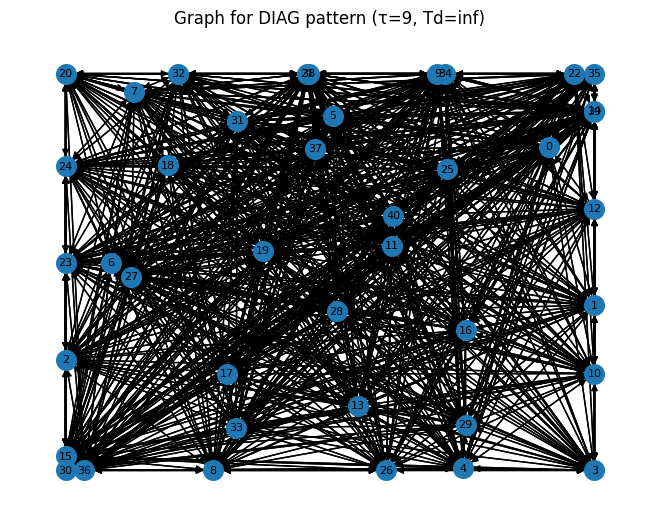
\includegraphics[width=3.5cm]{Graphics/japan-cluster-graph.png} \\ \hline
		Esquinas  & 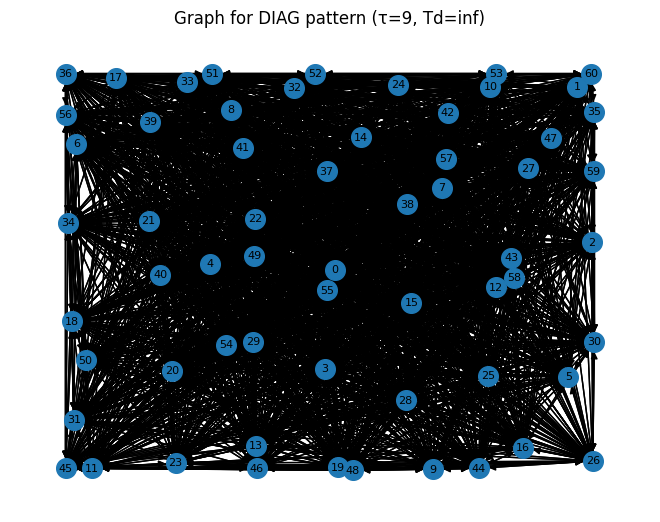
\includegraphics[width=3.5cm]{Graphics/disney-corner-graph.png} 
		& 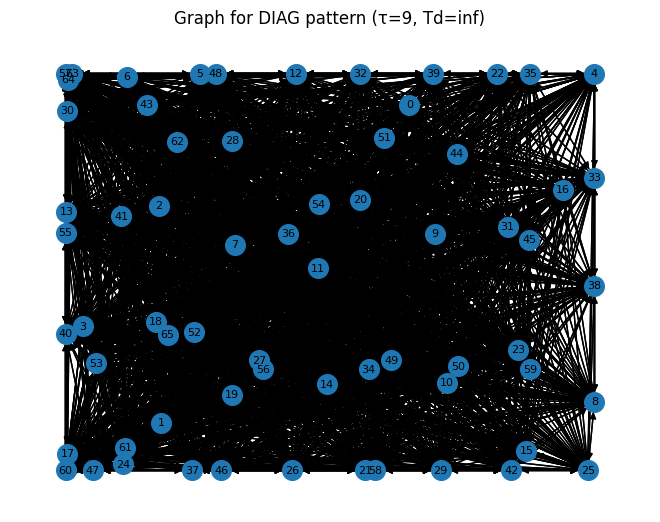
\includegraphics[width=3.5cm]{Graphics/cars-corner-graph.png} 
		& 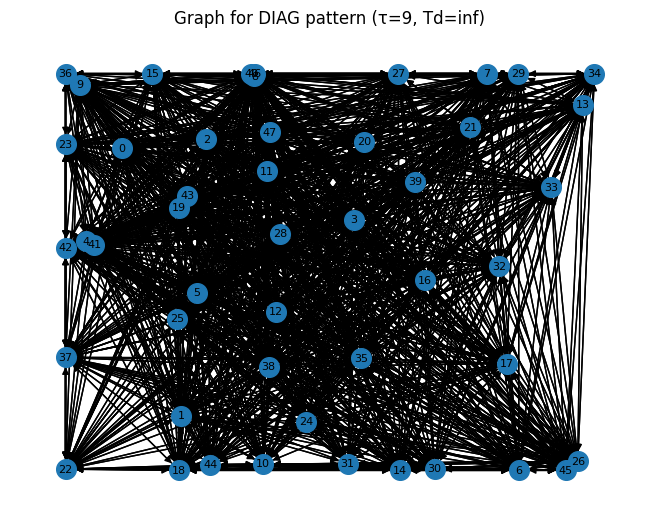
\includegraphics[width=3.5cm]{Graphics/japan-corner-graph.png} \\ \hline
		Saliencia & 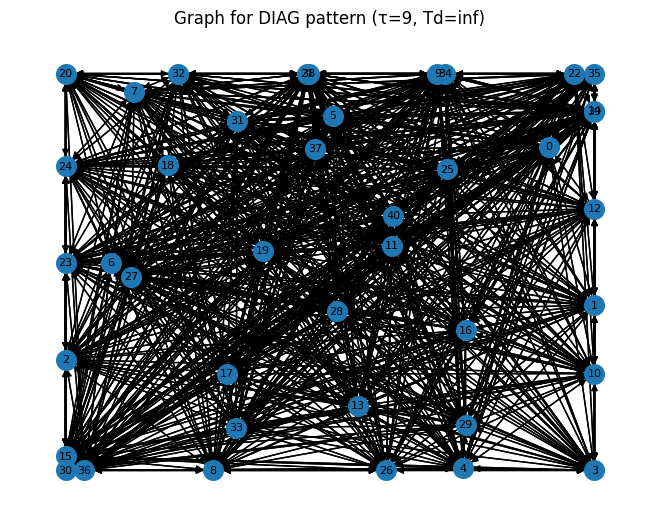
\includegraphics[width=3.5cm]{Graphics/disney-saliency-graph.png} 
		& 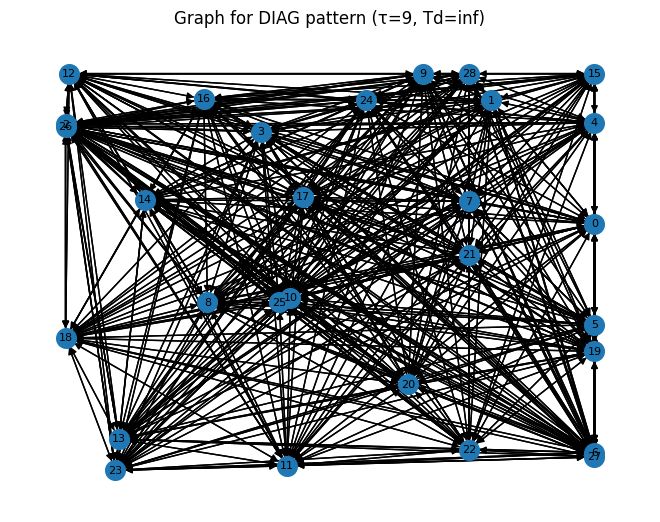
\includegraphics[width=3.5cm]{Graphics/cars-saliency-graph.png} 
		& 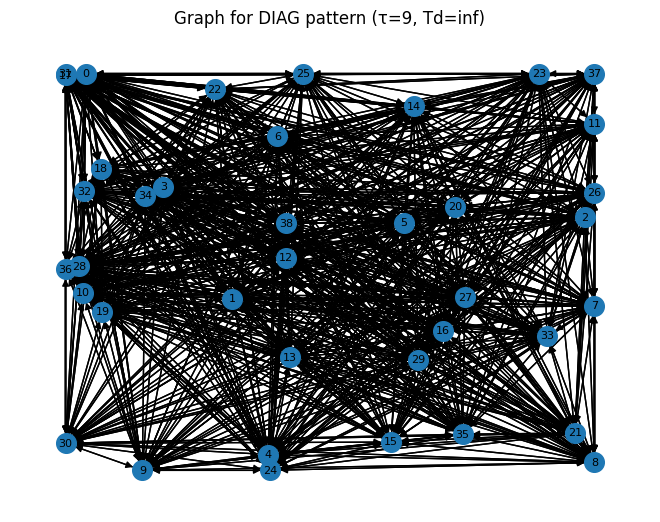
\includegraphics[width=3.5cm]{Graphics/japan-saliency-graph.png} \\ \hline
	\end{tabular}
	\caption{Grafos obtenidos para cada conjunto de puntos y el patr\'on DIAG}
	\label{graphs}
\end{table}


Para una mejor separaci\'on dichas heur\'isticas, se separaron los patrones en sub heur\'isticas, ver en \cite{van2010purely}, que disminuye la complejidad de implementar las comprobaciones de cada par de puntos. Luego para generar los diccionarios de ataque solo se necesita hallar los caminos de tama\~no 5 del grafo (ciclos inclu\'idos), en este caso se utiliz\'o DFS \textit{Depht First Search}, (B\'usqueda en profundidad), iterativo, guardando continuamente los resultados en archivos usando el formato \textit{JSON lines}. Esto permiti\'o reducir el requerimiento memoria ram por parte del sistema y tener una generaci\'on  din\'amica ya que el estado del DFS se guarda en el archivo. El tiempo de generaci\'on de dichos diccionarios oscil\'o de 2 a 3 horas cada uno, llegando a obtener archivos de 21GB de contrase\~nas, en la tabla \ref{dictionary:lengths} se pueden ver la cantidad de contrase\~nas generadas en cada diccionario.  

\begin{table}[H]
	\centering
	\caption{Tama\~no de los diccionarios obtenidos}
	\label{dictionary:lengths}
	\begin{tabular}{|l|l|l|l|l|l|l|l|l|l|}
		\hline
		\textbf{im\'agenes/contrase\~nas} & \textbf{segmentos} & \textbf{esquinas} & \textbf{saliencia }  \\ \hline
		\textbf{disney} & 14 880 348 & 389 469 380 & 104 960 000  \\ \hline
		\textbf{cars} & 1 114 112 & 558 134 287 & 17 825 024  \\ \hline
		\textbf{japan} & 5 387 888 & 3 894 822 & 81 320 304 \\ \hline
	\end{tabular}
\end{table}


\section{Ejecuci\'on del ataque}


Una vez generados los diccionarios, se procedió a la autenticación de cada usuario utilizando las contraseñas contenidas en los diccionarios de ataque. Para agilizar el proceso, esta tarea se realizó de manera asíncrona, como se ilustra en los ejemplos de código \ref{attack1} y \ref{attack}. No obstante, el ataque resultó infructuoso, ya que ninguna contraseña pudo ser vulnerada. Lo que significa que la muestra de las contrase\~nas seleccionadas por los usuarios no deben seguir patrones DIAG y LINE. Sin embargo, esto no quiere decir que est\'en absentas de alg\'un otro patr\'on no aleatorio. Por ende, en trabajos futuros se le a\~nadir\'a a la iplementaci\'on propuesta, los \textit{tests} existentes en la bibliograf\'ia para la detecci\'on de contrase\~nas que carezcan de aleatoriedad.
\bigskip\bigskip
\begin{lstlisting}[style=mystyle, language=Python, caption=C\'odigo del ataque, label=attack1][H]
data = (
supabase
.table('passwords')
.select('image, tolerance, user_id(email)')
.not_.is_('user_id', 'null')
.execute()
).data

results = {}

if not data:
 print("No se encontraron registros")
 exit()
threads=[]
for password in data:
  thread = Thread(target=predict_password,args=(password,))
  thread.start()
  threads.append(thread)
for thread in threads:
  thread.join()
\end{lstlisting}

\clearpage

\begin{lstlisting}[style=mystyle, language=Python, caption=C\'odigo que se ejecuta en cada hilo del ataque, label=attack][hb]
def predict_password(password):
 base_path = os.path.join("[ruta a las im\'agenes]", password['image'])  # Directorio base organizado
 email = password['user_id']['email'] if isinstance(password['user_id'], dict) else None

 #Aqui se guardar\'an los intentos de autenticaci\'on realizados
 with lock:
  results[email] = {
	'cluster_tries': 0,
	'corner_tries': 0,
	'saliency_tries': 0
  }

 file_types = {
	'saliency': 'saliency_dictionary.json',
	'cluster': 'cluster_dictionary.json',
	'corner': 'corner_dictionary.json'	
 }

 for key, filename in file_types.items():
  file_path = os.path.join(base_path, filename)
  with jsonlines.open(file_path) as points_data:
   for points in points_data:
     results[email][f'{key}_tries'] += 1

  passpoints = {
	'points': list(map(lambda x: {'x':x[0],'y':x[1]},points)),
	'tolerance': password['tolerance'],
	'image': {
		'name': password['image']
	}
  }

  # 8. Llamada a \textit{Supabase}  
  response = supabase.functions.invoke(
  "passpoints-login",
     invoke_options={
    	"body": {
		'email': email,
		'password': passpoints
 	  }
   }
  )
  resp = json.loads(response)
  if resp['success']:
   return {'success':True,'results':results[email]}
\end{lstlisting}

\backmatter

\begin{conclusions}
    Conclusiones
\end{conclusions}

\begin{recomendations}
   A partir de los resultados obtenidos en este trabajo y con el objetivo de continuar el desarrollo y mejora del sistema \textit{Passpoints}, se sugieren las siguientes recomendaciones para trabajos futuros:
   
   \begin{itemize}
   	\item 	\textbf{Análisis de correlación entre datos de usuarios y aleatoriedad de contraseñas}: Se recomienda estudiar la relación entre los datos recopilados de los usuarios y la aleatoriedad de las contraseñas gráficas que estos generan. Este análisis permitirá evaluar si existen patrones predecibles que puedan comprometer la seguridad del sistema.
   	
   	\item 	\textbf{Implementación de tests de aleatoriedad para contraseñas gráficas}: Se sugiere incorporar pruebas que permitan detectar patrones predecibles en las contraseñas gráficas. Estos tests, contribuirán a mejorar la robustez del sistema contra ataques de ingeniería social y fuerza bruta.
   	
   	\item 	\textbf{Mecanismo de detección de intentos de autenticación}: Se recomienda desarrollar un mecanismo capaz de reconocer los intentos de autenticación de un usuario legítimo y descartar aquellos provenientes de un atacante. Un posible enfoque para esta implementación es el modelo propuesto en \cite{legon2019nuevo}, el cual podría ser adaptado y evaluado en el contexto del sistema 	extit{Passpoints}.
   	
   	\item 	\textbf{Pruebas a mayor escala}: Para validar la viabilidad del sistema en escenarios reales, se sugiere realizar pruebas con una mayor cantidad de usuarios. Esto permitirá obtener datos más representativos y evaluar el rendimiento y la seguridad del sistema en entornos con alta concurrencia.
   	
   	\item 	\textbf{Uso de imágenes de mayor dimensión}: Se recomienda emplear imágenes de mayor resolución en el sistema, lo que podría incrementar el espacio de contrase\~nas y, en consecuencia, mejorar la seguridad general del método.
   	
   	\item 	\textbf{Ampliación del conjunto de imágenes}: Se sugiere incorporar una cantidad significativa de imágenes al sistema con el fin de diversificar las opciones disponibles para los usuarios y reducir la posibilidad de selección de puntos predecibles dentro de las mismas.
   	
   \end{itemize}
   
   Estas recomendaciones buscan fortalecer la seguridad y usabilidad del sistema \textit{Passpoints}, asegurando su efectividad como una alternativa viable a las contraseñas alfanuméricas tradicionales.
\end{recomendations}

\printbibliography[heading=bibintoc]

\begin{anexos}
	
	
	
	
	\begin{figure}[H]
		\centering
		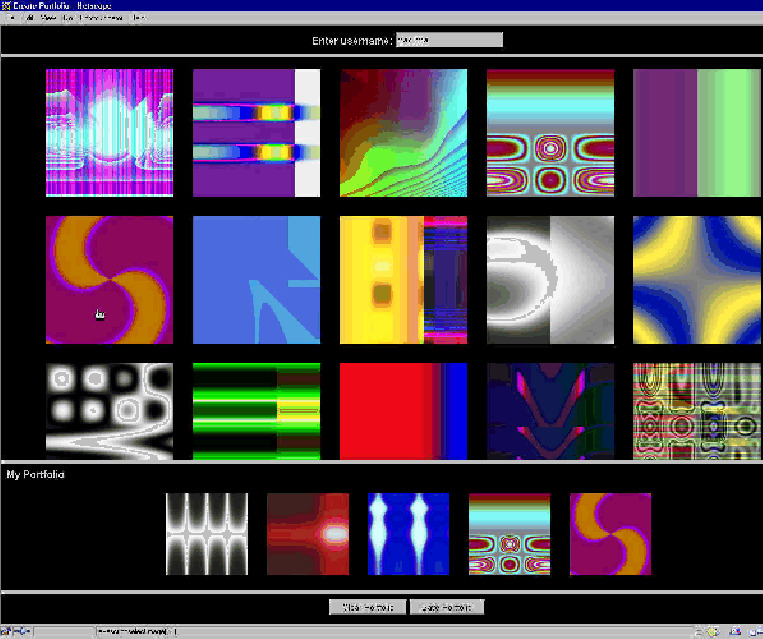
\includegraphics[width=0.5\linewidth]{Deja-Vu.jpg}
		\anexofigurecaption{Selección de portafolio. Fuente: \cite{dhamija2000deja}}
		\label{figure:deja-vu}
	\end{figure}


\begin{figure}[H]
	\centering
	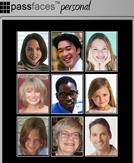
\includegraphics[width=0.3\linewidth]{3.jpg}
	\anexofigurecaption{Sistema PassFaces. Fuente: \cite{inproceedings}}
	\label{passfaces}
\end{figure}

\begin{figure}[H]
	\centering
	\begin{minipage}{0.5\linewidth}  % Tercer cuadrado, 48% del ancho de línea
		\centering
		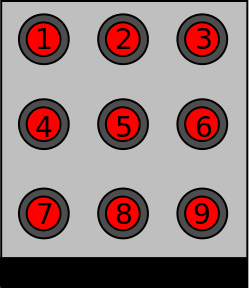
\includegraphics[width=0.7\linewidth]{0.png} % Imagen 3
	\end{minipage}%
	\hfill
	\begin{minipage}{0.5\linewidth} % Cuarto cuadrado, 48% del ancho de línea
		\centering
		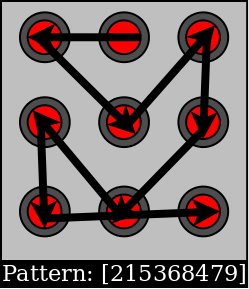
\includegraphics[width=0.7\linewidth]{1.png} % Imagen 4
	\end{minipage}
	\anexofigurecaption{Funcionamiento de un patrón de desbloqueo. Fuente: \cite{aviv2010smudge}}
	\label{android-pattern}
\end{figure}


\begin{figure}[H]
	\begin{minipage}{0.5\linewidth}  % Primer cuadrado, 48% del ancho de línea
		\centering
		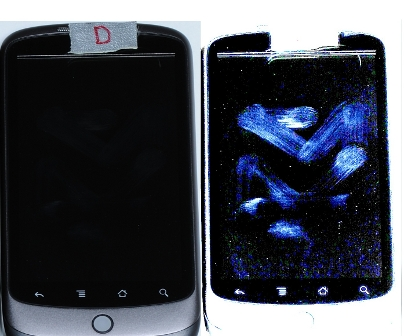
\includegraphics[width=\linewidth]{13.jpg} % Imagen 1
	\end{minipage}%
	\hfill
	\begin{minipage}{0.5\linewidth}  % Segundo cuadrado, 48% del ancho de línea
		\centering
		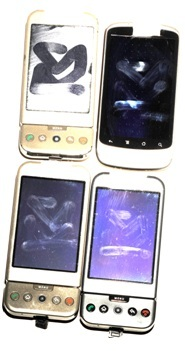
\includegraphics[width=0.5\linewidth]{9.jpg} % Imagen 2
	\end{minipage} % Espacio vertical entre filas

	\anexofigurecaption{Grasa en pantalla usada en los ataques de smudge. Fuente: \cite{aviv2010smudge}}
		\label{smudge-screen}
\end{figure} 

\begin{figure}[H]
	\centering
	\begin{minipage}{0.5\linewidth}  % Tercer cuadrado, 48% del ancho de línea
		\centering
		
\includegraphics[width=0.7\linewidth]{mouse.png} % Imagen 3
		\caption{Dibujado 6 veces usando el mouse. Fuente: \cite{lin2009free}}
		\label{free-draw-train-mouse}
	\end{minipage}%
	\hfill
	\begin{minipage}{0.5\linewidth} % Cuarto cuadrado, 48% del ancho de línea
		\centering
		
\includegraphics[width=0.7\linewidth]{stylus.png} % Imagen 4
		\caption{Dibujado 6 veces usando stylus. Fuente: \cite{lin2009free}}
		\label{free-draw-train-stylus}
	\end{minipage}
	
		\centering
	\begin{minipage}{0.48\linewidth}  % Tercer cuadrado, 48% del ancho de línea
		\centering
		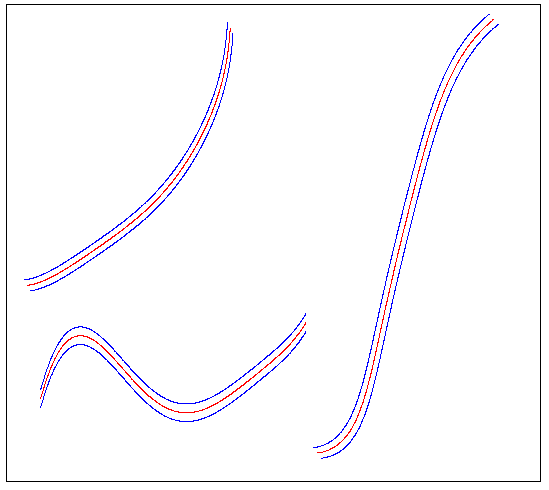
\includegraphics[width=0.9\linewidth]{polinomial.png} % Imagen 3
		\caption{Valores predichos e intervalos de predicción generados por el modelo de regresión polinomial. Fuente: \cite{lin2009free}}
		\label{free-form-draw-polinomial}
	\end{minipage}%
	\hfill
	\begin{minipage}{0.48\linewidth} % Cuarto cuadrado, 48% del ancho de línea
		\centering
		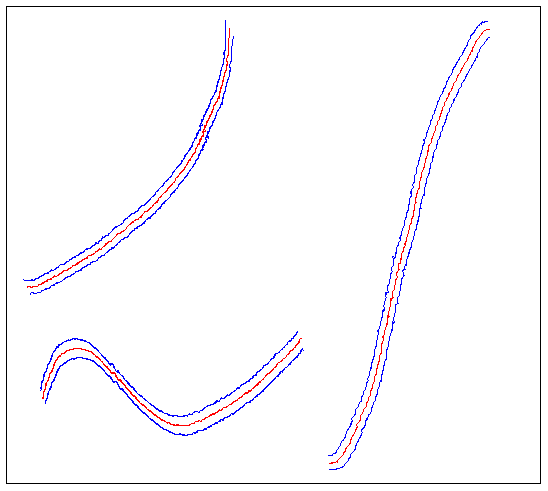
\includegraphics[width=0.9\linewidth]{b-spline.png} % Imagen 4
		\caption{Valores predichos e intervalos de predicción generados por el modelo de regresión B-spline. Fuente: \cite{lin2009free}}
		\label{free-form-draw-spline}
	\end{minipage}
	\anexofigurecaption{Valores predichos e intervalos de predicción generados por los modelos de regresi\'on. Fuente: \cite{lin2009free}}
	
\end{figure}




\begin{figure}[H]
	\centering
	\begin{minipage}{0.5\linewidth}  % Tercer cuadrado, 48% del ancho de línea
		\centering
		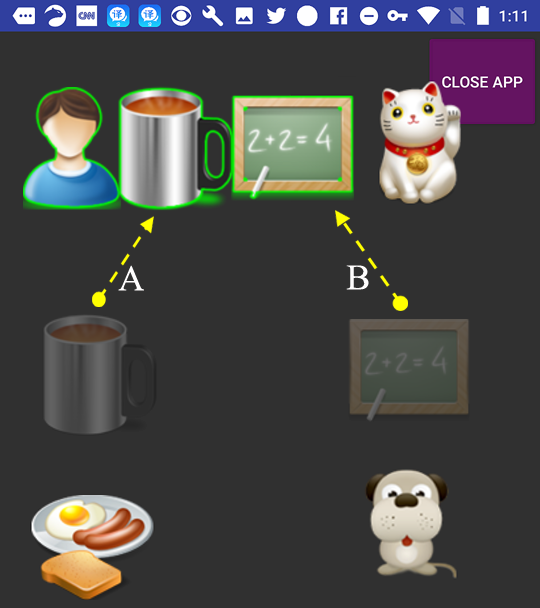
\includegraphics[width=0.8\linewidth]{semantoc-psw-2.png} % Imagen 3
		
	\end{minipage}%
	\hfill
	\begin{minipage}{0.5\linewidth} % Cuarto cuadrado, 48% del ancho de línea
		\centering
		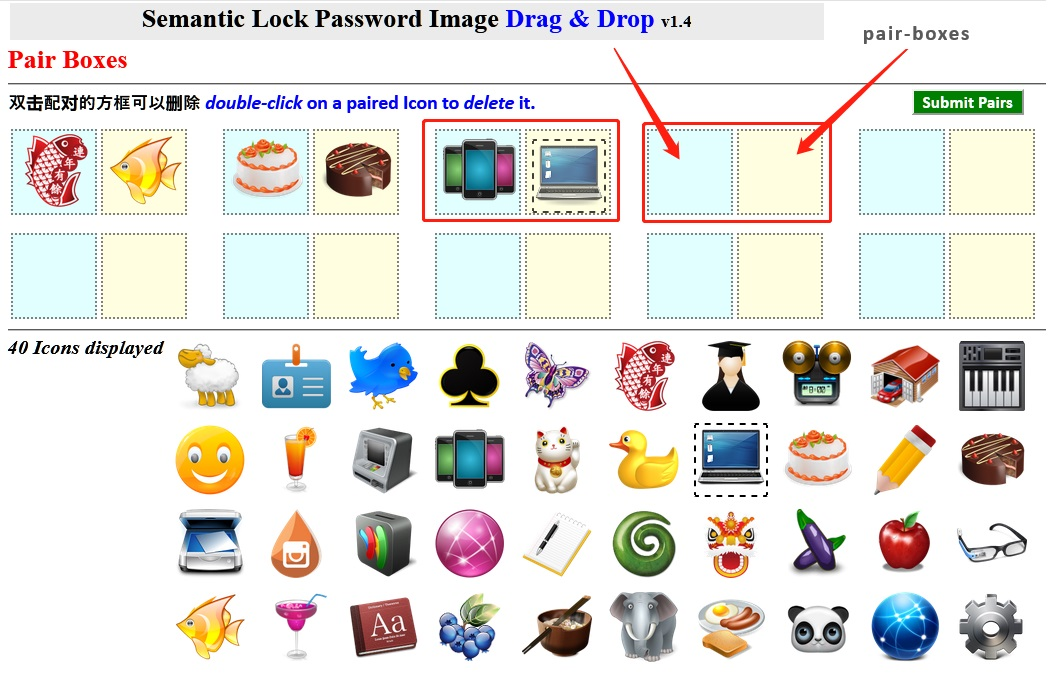
\includegraphics[width=0.8\linewidth]{semantic-psww1.jpg} % Imagen 4
		
	\end{minipage}
	\anexofigurecaption{Funcionamiento de Semantic Lock. Fuente: \cite{olade2023story}}
	\label{semantic-passw}
\end{figure}


\begin{figure}[H]
	 \centering
	\adjustbox{valign=b}{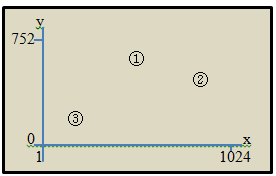
\includegraphics[width=0.8\linewidth]{pass-positions.png}} % valign=t para alinear la imagen en la parte superior
	\anexofigurecaption{Cálculo de hash de un punto Passpositions. Fuente: \cite{8320723}}
	\label{passpositions-example}
	
\end{figure}

\begin{figure}[H]
	\centering
	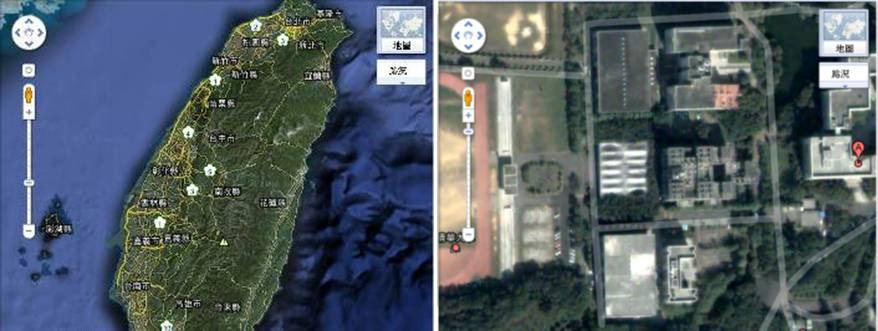
\includegraphics[width=0.5\linewidth]{pass maps2.jpg}
	\anexofigurecaption{Información del mapa en diferentes lugares y niveles de zoom. Fuente: \cite{10.1145/2414456.2414513}}
	\label{passmap}
\end{figure}

\begin{figure}[H]
	\begin{minipage}{0.4\linewidth}  % Primer cuadrado, 48% del ancho de línea
		\centering
		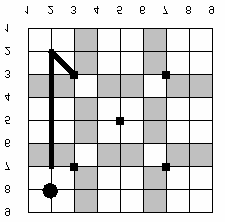
\includegraphics[width=\linewidth]{passgo1.png} % Imagen 1
	\end{minipage}%
	\hfill
	\begin{minipage}{0.4\linewidth}  % Segundo cuadrado, 48% del ancho de línea
		\centering
		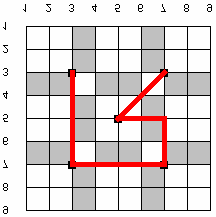
\includegraphics[width=\linewidth]{passgo2.png} % Imagen 2
	\end{minipage} % Espacio vertical entre filas
	\hfill
	\centering
	\begin{minipage}{0.4\linewidth}  % Segundo cuadrado, 48% del ancho de línea
		\centering
		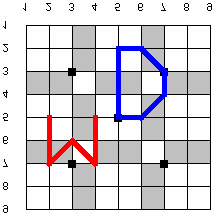
\includegraphics[width=\linewidth]{passgo3.png} % Imagen 2
	\end{minipage} % Espacio vertical entre filas
	\anexofigurecaption{Ejemplos de contraseñas usando Pass Go. Fuente: \cite{tao2008pass}}
	\label{go-passwords}
\end{figure} 



 \begin{figure}[H]
 	\begin{figure}[H]
 		\centering
 		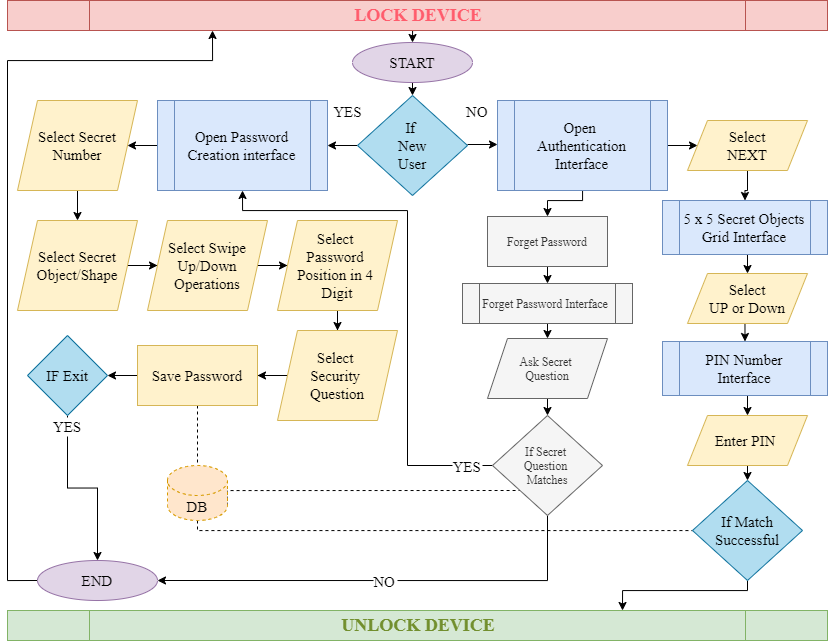
\includegraphics[width=0.6\linewidth]{grapin-proceso.png}
 		\caption{Proceso de autenticación \textit{Gra-Pin}. Fuente: \cite{kausar2022gra} }
 		\label{gra-pin}
 	\end{figure}
	\centering
	\begin{minipage}[b]{0.4\linewidth}  % Tercer cuadrado, 48% del ancho de línea
		\centering
		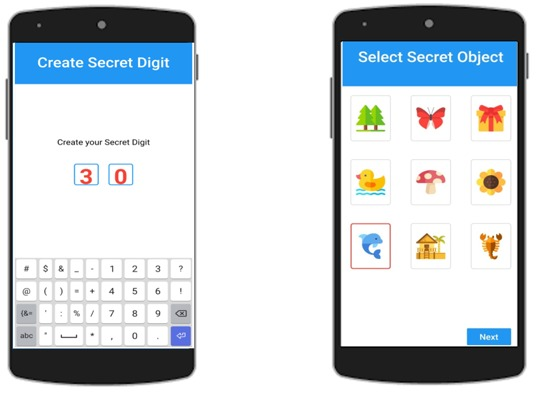
\includegraphics[width=\linewidth]{grapin-secret.jpg}
		\caption{Selección del número e imagen secretos. Fuente: \cite{kausar2022gra} }
	\end{minipage}%
	\hfill
	\begin{minipage}[b]{0.5\linewidth} % Cuarto cuadrado, 48% del ancho de línea
		\centering
		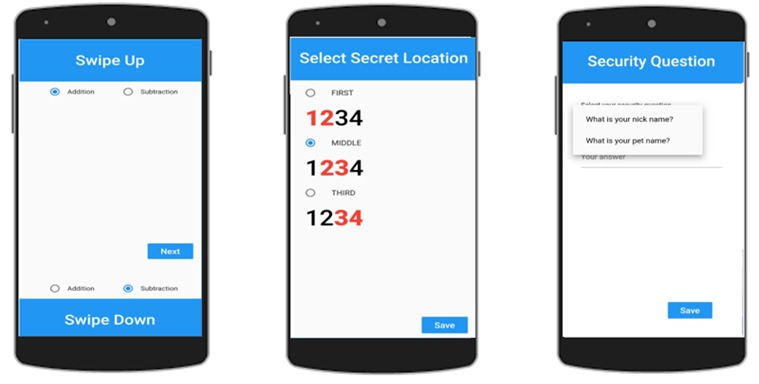
\includegraphics[width=\linewidth]{grapin-position.jpg}
		\caption{Selección de la operación y posición en el Pin de la clave. Fuente: \cite{kausar2022gra}  }          
	\end{minipage}
	\begin{minipage}[b]{0.4\linewidth} % Cuarto cuadrado, 48% del ancho de línea
		\centering
		\includegraphics[width=\linewidth]{grapin-auth.jpg}
		\caption{Pantalla de autenticación. Fuente: \cite{kausar2022gra}}
			\label{gra-pin-end}
	\end{minipage}
	\anexofigurecaption{Pantallas de autenticación de \textit{Gra-Pin}. Fuente: \cite{kausar2022gra}}
	\label{gra-pin-screens}
\end{figure}




%capturas
\begin{figure}

	\begin{minipage}[ht]{\linewidth}
			\centering
		\begin{minipage}[t]{0.48\linewidth}  % Tercer cuadrado, 48% del ancho de línea
			\centering
			\includegraphics[width=\linewidth]{Graphics/capturas/registro-landscape.png}
			\caption{Pantalla de registro en vista escritorio }
			\label{register-screen}
		\end{minipage}%
		\hfill
		\begin{minipage}[t]{0.48\linewidth} % Cuarto cuadrado, 48% del ancho de línea
			\centering
			\includegraphics[width=\linewidth]{Graphics/capturas/fullscreen-password-selector.png}
			\caption{Selecci\'on de imagen y contrase\~na a pantalla completa }   
			\label{full-screen-password}       
		\end{minipage}
	\end{minipage}
		

	

	\begin{minipage}[ht]{\linewidth}
			\centering
		\begin{minipage}[t]{0.48\linewidth}  % Tercer cuadrado, 48% del ancho de línea
			\centering
			\includegraphics[width=\linewidth]{Graphics/capturas/profile.png}
			\caption{Perfil del usuario para recaudar informaci\'on }
			\label{user-profile} 
		\end{minipage}%
		\hfill
		\begin{minipage}[t]{0.48\linewidth} % Cuarto cuadrado, 48% del ancho de línea
			\centering
			\includegraphics[width=\linewidth,height=4cm]{Graphics/capturas/notes.png}
			\caption{Vista de notas para dejar valoraciones } 
			\label{notes}          
		\end{minipage}
		\end{minipage}

	\begin{minipage}[hb]{\linewidth}
		\centering
	\begin{minipage}[b]{0.6\linewidth}  % Tercer cuadrado, 48% del ancho de línea
		\centering
		\includegraphics[width=\linewidth]{Graphics/capturas/full-screen disney-password.png}
		
	\end{minipage}%
	\hfill
	\begin{minipage}[b]{0.3\linewidth} % Cuarto cuadrado, 48% del ancho de línea
		\centering
		\includegraphics[width=0.5\linewidth,height=5cm]{Graphics/capturas/password-mobile.png}
		
	\end{minipage}
	
	
	\caption{Misma contrase\~na en diferentes tama\~nos de pantalla }
	\label{screen-shapes-variety}
	\end{minipage}

\begin{minipage}[hb]{\linewidth}
		\centering
\begin{minipage}[hb]{0.6\linewidth}  % Tercer cuadrado, 48% del ancho de línea
	\centering
	\includegraphics[width=\linewidth]{Graphics/capturas/cars-login-error-landscape.png}
	
\end{minipage}%
\hfill
\begin{minipage}[hb][0.3\linewidth]{0.2\linewidth} % Cuarto cuadrado, 48% del ancho de línea
	\centering
	\includegraphics[width=0.7\linewidth,height=4.8cm]{Graphics/capturas/login-error-mobile.png}
	
\end{minipage}
\caption{Misma contrase\~na incorrecta en diferentes tama\~nos de pantalla }
\label{error-scans}
\end{minipage}

		\anexofigurecaption{Diferentes vistas de la aplicaci\'on}
\end{figure}




\end{anexos}


\end{document}